\documentclass{../tex/report}
\usepackage{setspace} % Setting line spacing
\usepackage{ulem} % Underline
\usepackage{caption} % Captioning figures
\usepackage{subcaption} % Subfigures
\usepackage{geometry} % Page layout
\usepackage{multicol} % Columned pages
\usepackage{multirow}
\usepackage{array,etoolbox}
\usepackage{fancyhdr}
\usepackage{enumitem}
\usepackage{tabularx}
\usepackage[toc,page]{appendix}
\setlist{noitemsep}

% Page layout (margins, size, line spacing)
\geometry{letterpaper, left=1in, right=1in, bottom=1in, top=1in}
\setstretch{1}

% Headers
\pagestyle{fancy}
\lhead{PeaPod - Final Report}
\rhead{PeaPod Technologies Inc.}

\begin{document}

\begin{titlepage}
    \begin{center}
        \vspace*{1.2cm}

        \textbf{\large{PeaPod - Final Report}}

        \vspace{0.5cm}

        NASA/CSA Deep Space Food Challenge Phase 2

        \vfill
        \small{
    \textbf{Jayden Lefebvre - Founder, Lead Engineer}\\
    Port Hope, ON, Canada\\
    \vspace{.5cm}
    \textbf{Nathan Chareunsouk - Design Lead}\\Toronto, ON, Canada\\
    \vspace{.5cm}
    \textbf{Navin Vanderwert - Design Engineer}\\
    BASc Engineering Science (Anticipated 2024), University of Toronto, Toronto, ON, Canada\\
    \vspace{.5cm}
    \textbf{Jonas Marshall - Electronics Engineer}\\
    BASc Computer Engineering (Anticipated 2024), Queen's University, Kingston, ON, Canada\\
    \vspace{.5cm}
    Open-source contributions made by:\\
    \textbf{University of Toronto Agritech}
}

\vspace{1cm}

Primary Contact Email: contact@peapodtech.com
        \vspace{.75cm}

        Revision 0.2\\
        PeaPod Technologies Inc.\\
        January 31st, 2023

    \end{center}
\end{titlepage}

\thispagestyle{plain}

\tableofcontents
\newpage

\section{Technology Description and Progress}
% How does it work?
% What is novel, sustainable, and innovative?
% What foods does it create?
% How are you minimizing inputs and maximizing outputs?

% With a focus on progress or changes made during Phase 2 of the challenge, describe what the food production technology is, what it does, how it functions, and how the crew will interact with it. Include descriptions of major hardware components and processes. (limit 4000 characters).

PeaPod is an automated plant growth environment, made of control systems and an automation/monitoring system within a modular, cubic housing. It can generate any desired environment while collecting data on plant growth and improving yields.

NOTE: For this submission, only the 4x3 unit \textbf{Standard Extended PeaPod} is in consideration. It has one control module, and eight of each tray (grow and lighting).

PeaPod's control systems are made of environmental controls (feedback loops with sensors) and plant inputs (set-states):
\begin{itemize}
    \item\textit{Lighting}: LEDs, from near-ultraviolet to near-infrared. Dimmable drivers for precision spectrum and intensity control. Efficient, precise emission spectrum, low heat.
    \item \textit{Aeroponics}: Reverse osmosis (RO) water is pressurized by a pump (with sensor for safety cutoff), brought to temperature, nutrient-dosed and pH-balanced by Venturi siphons with servo-actuated flow control, and forced through nozzles to generate mist. Runoff water is recycled. Water-efficient (98\% less than farming), nutrient-efficient (60\% less), no pH/nutrient "feedback" (common in reservoir-based hydroponics), increased root oxygenation \cite{aeroponics}.
    \item \textit{Air Thermoregulation}: Leaf zone air temperature is regulated by a thermoelectric heat pump. Fans blow air over heat sinks connected to either face of a Peltier tile to circulate air and dissipate heat. A Proportionate-Integral-Derivative (PID) control system is informed by temperature sensors, and controls the direction and magnitude of the heat transfer. Low complexity, high safety/reliability, easy to automate (bidirectional, precisely dimmable, PID tuning).
    \item \textit{Humidity Regulation}: Leaf zone humidity is regulated by a dead-zone bang-bang control system informed by humidity sensors.
    \begin{itemize}
        \item \textit{Humidification}: RO water is supplied to a tank with a fine mesh piezoelectric disc. A controllable driver circuit oscillates the disk, producing water vapour. Easy to automate.
        \item \textit{Dehumidification}: A dry silica gel bead cartridge is covered by servo-actuated "shutters" to control dehumidification. Fans draw humid air through a HEPA filter into the desiccant and back into the growth environment. The beads change color to indicate water saturation. The crew is then notified to swap and "recharge" in a standard oven.
    \end{itemize}
    \item \textit{Aeroponic Water Temperature}: Root zone air temperature is regulated in the same way as the leaf zone system. Exceptions include an aluminum water block (vs internal heat sink and fan) and a single temperature sensor after the block for PID feedback in a flowing system.
    \newpage
    \item \textit{Gas Composition}: Oxygen and carbon dioxide levels are managed by gas exchange. Input and output ports allow fans to draw air into and out of the system. HEPA filters remove microbes and aerosols, and servo-actuated "shutters" prevent unintended exchange. Gas concentration sensors inform a bang-bang control system for port activation.
\end{itemize}

% Food products are optimized via plant metric analysis and machine learning. Two cameras (birds-eye and horizontal) provide data from which metrics of both plant health and yield quality are extracted. These, along with data collected on the environment, train a machine learning model to be a "digital representation" of the plant, treating environment and metrics as in/outputs to a "surrogate model". As more iterations of the plant species are grown, the dataset becomes generalized across environmental inputs/programs, and new ones can be selected via "gradient ascent" to target optimization factors (i.e. yield mass, flavour, nutrient concentration, energy/water efficiency).

Once PeaPod has been assembled, the first step is manual sterilization to prevent microbial growth at high growth environment humidities. Any plant- and food-safe means may be employed (i.e. UV, wipe-down with disinfectant followed by distilled water).

Next is the hookup of power, network, and water reservoir inputs, as well as the filling of the water reservoir (reverse osmosis, nutrient-rich and pH-balanced for crop choice).

PeaPod's operation begins at planting. Seeds are removed from vacuum-sealed storage bags and distributed evenly on mesh media, which is then moistened for germination and placed in the grow tray. The front panel is then closed, sealing the internal environment. Once sprouted, plants may be harvested as microgreens or transplanted to neoprene pucks inside grow cups for further growth.

The desired state of the growth environment is encoded via a standardized set of "environment parameters". The specific values of each parameter for each iteration are stored in a "program". The program is set prior to the start of plant growth, and consists of a set of \textbf{actions} (e.g. set red LEDs to 63\% power) and \textbf{control targets} (e.g. hold air temperature at 22°C) as time-series instructions from the start of planting to the point of harvest (or plant death, in the case of multiple-harvest plants) corresponding to the control systems.

When activated, PeaPod's control systems begin to enact the program. PeaPod will notify crew of any required action, including refilling inputs, cleaning components, and harvesting, as well as "End-of-Program", when all inedible plant matter is disposed of. The process can then be repeated (starting at sterilization).

\section{Adherence to Constraints}

\subsection{Volume}
% 100chars

\textbf{Constraint}: \textit{Fits through 1.07m x 1.90m doorway; W < 1.820m, D < 2.438m, H < 2.591m; V<= 2m${}^3$}

\textbf{Standard Expanded PeaPod}: 4x3x1 units = 194cm x 146cm x 50+20cm (DIN backplane) = 1.98m${}^3$ (< 2)

% With width treated as depth for the purposes of the considerations of the "room size" constraint, the Standard meets this constraint.

\subsection{Power}
% 1000chars

\textbf{Constraint}: \textit{Avg < 1500 W, Peak < 3000 W}

\textbf{Standard Expanded PeaPod}: Two Pumps (120W ea.), 4 Solenoids (36W ea.), LEDs at full power (8.4W per strip), 5 LED strips per grow tray = 849W

% For calculations and justification, see preliminary calculations Appendix \ref{app:power}.

\subsection{Water Consumption}
% limit 1000 characters
% CNet = (Initial water input + water added over time + water used for cleaning – condensed/ transpired water provided back to crew)

\textbf{Unconstrained}

% For calculations and justification, see preliminary calculations Appendix \ref{app:water}.

\textbf{Standard Expanded PeaPod}: Dependent on watering cycle, 5mL/sec per nozzle @100PSI.

For 10sec watering every 30min: CNet = \textbf{20L primed + 0.8L per hour} (without recycling).

\subsection{Mass}
% limit 1000chars

% For part breakdown, calculations, and justification, see preliminary calculations Appendix \ref{app:mass}.

\textbf{Standard Expanded PeaPod}: \textbf{90kg}

\subsection{Data Connection}
% limit 1000 characters

\textit{Automation}: All of PeaPod's operation is automated, save for a select few setup, maintenance, and harvest tasks. This is controlled by a central computer, which uses a "program" to enact the desired environment at each point in time throughout the plant life cycle. 
\textit{Remote Control}: The program may be changed \uline{instantaneously} as an \textbf{appended instruction set} with immediate effect.
\textit{Feedback}: The feedback sensors provide the computer with information that will influence the control it exerts. For example, if the program indicates the leaf zone temperature should be set to 22 degrees C, the computer would apply greater power to the heater if the current temperature was 18 degrees C as opposed to 21 degrees C. This forms a control loop for each parameter, relying on one of many control functions (bang-bang, PID, etc.).

% \textit{Data Presentation}: Plant and environment data can be viewed with \uline{live updates and video feed}.

\subsection{Crew Time}

\textbf{Constraint}: \textit{4 hrs/week}

For calculations and justification, see preliminary calculations Appendix.

Total setup process time (8 trays, 12 units, 1 CM): \textbf{17.5 hours} (\textit{one person}) or \textbf{4.5 hours} (\textit{crew of 4})

Total maintenance time per week: \textbf{2 hours} (depending on program)

\subsection{Operational Constraints}

\textbf{Constraint}: \textit{Terrestrial: gravity (9.81 m/s${}^2$), ambient atmospheric pressure (101,325 Pa), ambient atmospheric temperature (22 °C), ambient atmospheric humidity (50 \%RH)}

Design operates in terrestrial conditions.

Ambient pressure: tank, bladder, and nozzle are designed to produce indicated outputs at standard air pressure
Ambient temperature and humidity: less concern, housing is sealed and insulated

\section{Design Approach and Innovation}
% With a focus on the progress or changes made during Phase 2 of the challenge, outline how the design approaches the problem of food production technology for spaceflight in a novel of innovative manner. (limit 2000 characters)
% More specifically:
% How is your food production technology different from the currently available technology used for food production?
% What are the innovative or novel elements of your food production technology?

\textbf{Control Range and Parameter Independence}

Unlike large-scale vertical farming, PeaPod’s isolation and parameter independence lets it simulate any climate. Wide LED spectrum can emit both near-infrared and near-ultraviolet light, important for creating hormonal responses and compounds in plants. Combined with insulation, humidification and dehumidification, and thermoelectric heating/cooling, PeaPod can generate extreme environments and even conditions on other planets (minus gravity and atmospheric changes). 

These parameters are independent: e.g., lighting heat is countered by thermoregulation cooling. Also, inline nutrient and pH solution injection eliminates drawbacks of reservoir use by taking less space, less solution mixing time, and avoiding a control loop of nutrients/pH (while also being more accurate). 

%These innovations allow PeaPod to grow virtually any plant. 

\textbf{Form Factor and Extendability}

The range of output environments is also possible because of the form factor of a single PeaPod unit. Warehouse-scale vertical farming cannot provide wide-spectrum control due to size---poor insulation and air circulation prohibits extreme temperatures. PeaPod solves this with a small, modular design that enables robust lighting, heating, and cooling systems at home and at scale.

Space savings are a benefit of this feature, as the output of an entire farming or hydroponics setup (requiring a flat field or warehouse) can be spread through unused space (corners, under shelves/desks, etc.) via many small PeaPod setups. This means a large yield can be had without construction, zoning, labour, or any of the other issues accompanying large farming or hydroponic setups.

\textbf{Optimization}

Existing approaches to plant optimization are simple and ineffective, relying on a \textbf{fixed/unchanging} environment parameter set and only examining \textbf{final} plant metrics. This approach is severely limited, in that it does not account for changes over time.

Instead, statistical model is used which takes into account the cumulative property of growth. By monitoring all environment and plant indicators, repeatable and controlled trials with scientific validity are able to be performed. PeaPod counters declining health/quality indicators in real time, and generates tailored programs that to maximize any metric and target further improvement.

% See the preliminary calculations Appendix \ref{app:optimization} for details.

\textbf{Open-Source Design and Data}

Since PeaPod is standard and open-source, units can be had in bulk and assembled by anybody. Public contribution to the project (both in design improvement and data) increases the reliability and safety of the solution. Collected data is, ideally, committed to the public, meaning anybody with a PeaPod can run the same iteration with the same program and species to boost scientific validity, or run a different program to expand PeaPod's knowledge base.

\section{Scientific and Technical Merit}
% With a focus on the progress or changes made during Phase 2 of the challenge, explain how your proposed food production technology demonstrates scientific and technical merit. (limit 4000 characters)
% More specifically:
% Outline your objectives, approaches, and plans you created for developing and verifying the food production technology.
% Please describe your scientific and technical methodology.

\section{Feasibility of Design}
% With a focus on the progress or changes made during Phase 2 of the Challenge, please describe how your technical approach is technically and realistically feasible for use in future space missions (limit 4000 characters).
% More specifically:
% Describe how the related operation processes and procedures are technically and realistically feasible, including (but not limited to):
% Food production
% Food handling
% Maintenance
% Repair
% What alterations would need to be made to make your food production technology feasible in a space flight environment?
% Ensure the emphasis is on future space missions.

% Are there any risks that your food production technology may pose in future space missions, and what are your proposed solutions to mitigate these risks? (limit 2000 characters)

\section{Terrestrial Potential}
% With a focus on the progress or changes made during Phase 2 of the challenge, please outline how the food production technology has the potential to improve terrestrial food production. (limit 10000 characters)
% This may include but is not limited to: Improved cost-benefit, quality and shelf-life of food for harsh and isolated environments, greater and improved food production for food deserts in mild environments and urban centers, new rapid-deployment technologies for humanitarian responses to disasters, and energy used in an efficient way and/or improved process control using e.g. machine learning

% \textbf{Customer-facing Food Service} %OpenComment does this make sense? feels a little weak/unfounded - NV

% A restaurant serving fresh produce needs either a local supplier or a substantial amount of outdoor space. Both of these are cost-prohibitive, and the latter is impossible in many urban situations. Local suppliers' high costs are the result of a few things:
% \begin{itemize}
%     \item Limited seasonal availability
%     \item Frequent transport need
%     \item High costs with little demand
% \end{itemize}
% PeaPod has the potential to reduce these barriers in a cyclic way. Partnerships between local suppliers and restaurants will provide these restaurants with space- and time-efficient PeaPod units with the purpose of generating both produce and data. The increase in produce will reduce the frequency at which suppliers need to make deliveries (reducing cost and spreading demand), while the data generated will let suppliers maximize output, quality, and longevity. Over time, this increases efficiency to the point where local suppliers can provide produce at a lower price, increasing the presence of fresh, local, produce in cities worldwide.

% Another food service application of PeaPod is the globalization of otherwise endemic crops. For example, Wasabi is a difficult-to-grow Japanese crop that is near-impossible to grow overseas (save a few recent commercial developments). PeaPod units in restaurants solve this issue by re-creating the necessary precise conditions and eliminating barriers in skill and time that otherwise impact Wasabi's production and consumption overseas. And, of course, PeaPod's data collection capabilities can be harnessed by farmers to discover more safe, efficient, and adaptable methods of producing crops such as these.

\textbf{Agriculture-as-a-Service}

PeaPod’s modularity and ease of storage can turn unused city spaces to PeaPod farms. With fresh produce in local areas, PeaPod can be a direct food system to paying customers. A subscription service would provide patrons with fresh produce without a middle man. By eliminating transport, distribution, and grocery stores, PeaPod creates fresher, better produce for the general public at a lower cost.

\textbf{Crowd-Sourced Research}

PeaPod's automation is unique in the research space, allowing for autonomous, off-site research. Universities save costs related to space and energy usage by subsidizing PeaPods to individuals, schools, or even restaurants. Users receive sets of parameters to grow crops with, sending data back to the institution and using the produce at the cost of space and energy. The result is a massive dataset from identical conditions in different places, verified by comparison with devices conducting the same tests.

This is an effective tool in climate change famine aid. By predicting conditions in at-risk areas, researchers can conduct tests ahead of time to determine what seeds, traits, and care parameters are most effective for certain conditions. This also informs development of seeds specialized for extreme climates, letting areas counteract food scarcity by having a variety of options prepared ahead of time.

\textbf{De-centralized Production}

Many crops are endemic to certain climates, making global transport necessary to for foreign markets. This reduces freshness, necessitates preservatives, and increases the carbon footprint of agriculture. By upscaling PeaPod technology to a farm scale, climate-bound crops can be produced anywhere. This creates regional farms of global variety, making it easier to have a local food diet.

PeaPod's form factor makes it a viable tool for at-home production, either in cities or off-grid. With only a solar power source, water, and a compact supply of nutrient solutions, users can sustain crops even through winter without travelling for nutrients and supplies.

% \textbf{Blockchain and "PlantCoin" Cryptocurrency Mining}

% In the same way current cryptocurrencies reward nodes for validating all information on a blockchain, a PeaPod network would reward nodes (individual PeaPods) for validating data produced by other nodes. When tens or hundreds of units produce statistically similar results in independent trials using the same parameters, all units are rewarded for their contribution to the network. This process is commonly known as "mining". This allows consumers the option to operate a PeaPod as a passive source of income, with the unit paying for itself by both producing food and mining a "PlantCoin" cryptocurrency.

% This also incentivizes the network to find critical points in the n-dimensional set of data that would otherwise not be checked. For example, few users would intentionally grow plants in drought conditions at this will produce subpar produce. But, by incentivizing users to fill sparse sections of data, we can generate information critical to developing crops for territories affected by climate change.

%we love this idea but idt nasa cares

\textbf{Food Infrastructure Micro-Loans}

For many, finding fresh produce is a struggle whilst growing your own is prohibitively expensive. Micro-loan platforms have attempted to solve this by letting donors fund an interest-free loan for technology/infrastructure which then pays the loan as a percentage of its surplus. 

Unfortunately, these are only feasible for individuals in rural areas with arable land and climate.

PeaPod brings this solution to low-income urban areas with a platform for donors to micro-loan PeaPod units and inputs. The user feeds themselves and sells surplus, while a percentage of sales go to the interest-free loan. Once paid, PeaPod continues to produce food while sales fund its operation. 

This creates permanent, self-sustaining agricultural infrastructure that pays for itself as it grows, requiring little initial capital. This means entire farms throughout high density buildings generating yield with little lost space and almost no labour.

\section{Results}

\subsection{Acceptability of Process}
% Teams must demonstrate the operations processes and procedures, including (but not limited to):
% Operational footprint (i.e., how much space is needed for the solution and its related processes?)
% Food production technology set up
% Food production cycle, including steps to produce food products
% Food handling, processing procedures and collection of food products
% Shutdown, cleaning, maintenance, repair and/or stowage procedure(s)
% An estimate of the overall crew time to operate and maintain the technology
%  (limit 10000 characters):

\textit{Footprint}:

Due to PeaPod's modular construction, the footprint can vary. For a Standard Extended PeaPod, the footprint would be 2m x 0.5m, or about three standing refrigerators. When stowed, volume is reduced to 37\% of when assembled. Control module is packed pre-assembled.

The following estimates are for a Standard Extended PeaPod.

\textit{Setup Process}:

\begin{enumerate}
    \item Assemble housing - \textbf{2 hours}
    \item Install control module(s):
    \begin{enumerate}
        \item Hook up water, power, and network inputs - \textbf{5 min}
        \item Fill nutrient and pH adjustment solution containers - \textbf{10 min}
        \item Mount CM to housing - \textbf{5 min}
    \end{enumerate}
    \item Assemble all trays - \textbf{1 hour},
    \item For each tray, either:
    \begin{enumerate}
        \item Mount lighting boards and driver, daisy chain boards to driver, hook up power and signal to driver and CM - \textbf{10 min} per tray, \textbf{OR}
        \item Mount aeroponic nozzle mount and arm, hook up water delivery line to nozzles and CM - \textbf{10 min} per tray
    \end{enumerate}
    \item UV sterilization - \textbf{20 min}
    \item Prepare and plant seeds for desired crop output, seal growth environment - \textbf{30 min}
    \item Enable primary power supply, and power on automation system, allow to perform self-test and calibrations - \textbf{10 min}
    \item Open water input shutoff valve
    \item Input program for required environments and activate - \textbf{5 min}
\end{enumerate}

Total setup process time (Standard: 2 trays per unit, 12 units, 1 CM): \textbf{8.5 hours} (\textit{one person}) or \textbf{2.5 hours} (\textit{crew of 4})

\newpage

\textit{Food Production Cycle}:

\begin{enumerate}
    \item Environment is maintained, and environment can be observed live at a computer terminal via sensor data and camera feed
    \item Circulation fans enable automated pollination
    \item Perform maintenance, including:
    \begin{itemize}
        \item Cleaning nozzle once a month - \textbf{10 min}
        \item Swapping and recharging dehumidification cartridges when instructed - \textbf{5 min} (active time)
        \item Refilling solution containers when instructed - \textbf{5 min}
    \end{itemize}
    \item Upon End-Of-Program (EOP) notification, the gas exchange system will conduct a "full equalization flush", bringing the internal environment in equilibrium with the surroundings. Users will harvest and store food products (or prepare and consume them immediately, varying time) - \textbf{15 min}
    \item All organic material remaining in the system is removed and disposed of, presence of residue or algae is determined - \textbf{10 min}
    \item If algae present, hydrogen peroxide is used to kill the growth - \textbf{5 min}
    \item (Optional) In event of significant contamination, system can be flushed with an all-purpose surface disenfectant and then rinsed with distilled water - \textbf{10 min}
    \item Upon End-Of-Life notification (may occur at the same time as EOP), the plant is scrapped (\textbf{15 min}), and new plants may be planted
\end{enumerate}

Total maintenance time per week: \textbf{1-2 hours} (depending on program)

\textit{Process Evaluation}:

Setup and maintenance processes are fully documented in a "User Manual", which includes both text instructions (with numerical specifications for different actions) as well as diagrams for reference. Notifications from computer refer users to specific subsections of the Manual for maintenance actions. All processes require no specific expertise, just the ability to operate basic hand tools and follow instructions.

All interactions with the automation system (i.e. program upload, environment/camera monitoring) can be accomplished either via a touchscreen panel on the front of the control module or over the Internet.

\subsection{Acceptability of Product}
% Please provide an assessment (using industry standards and existing research) that the food outputs of their technology are likely to meet the acceptability target/rating described. This assessment should include the palatability of the food product (appearance, aroma, texture and flavour) (limit 6000 characters).

There are several considerations when examining the acceptability of the products of our system:

\begin{enumerate}
    \item Produce is not only eaten fresh, but also forms the basis for an innumerable variety of combined and prepared foods (i.e. fresh tomatoes vs. tomato sauce);
    \item When considering prepared derivatives of the food products, the quality of the preparation is a key factor in acceptability. As such, proper care in training and is to be taken;
    \item The products formed by the system (and their properly prepared derivatives) are not exceptional or novel. They are the same plant-based foods grown, consumed, and \textbf{accepted} terrestrially, just grown in a more efficient and controlled way. As such, their acceptability is determined to be of \textbf{equal or greater value};
    \item Plant-environment optimization can be targeted not only at nutritional value or efficiency, but also at acceptability. The feedback can be gathered either through crew Hedonic rating (i.e. tomatoes grown in environment ABC rate X in appearance, Y in aroma, etc.) or more sophisticated analysis (i.e. computer vision analysis of color/size/shape for appearance, tissue concentrations of various aroma/flavor compounds); %TODO: cite some times when this has been performed, i.e. MIT basil study
\end{enumerate}

\section{Safety}

\documentclass{report}
\usepackage{setspace} % Setting line spacing
\usepackage{ulem} % Underline
\usepackage{caption} % Captioning figures
\usepackage{subcaption} % Subfigures
\usepackage{geometry} % Page layout
\usepackage{multicol} % Columned pages
\usepackage{array,etoolbox}
\usepackage{fancyhdr}
\usepackage{enumitem}
\usepackage[toc,page]{appendix}
\setlist{noitemsep}

% Page layout (margins, size, line spacing)
\geometry{letterpaper, left=1in, right=1in, bottom=1in, top=1in}
\setstretch{1}

% Headers
\pagestyle{fancy}
\lhead{PeaPod - Testing Plan}
\rhead{PeaPod Technologies Inc.}

\begin{document}

\begin{titlepage}
    \begin{center}
        \vspace*{1.2cm}

        \textbf{\large{PeaPod - Testing Plan}}

        \vspace{0.5cm}

        NASA/CSA Deep Space Food Challenge Phase 2

        \vfill
        \small{
    \textbf{Jayden Lefebvre - Founder, Lead Engineer}\\
    Port Hope, ON, Canada\\
    \vspace{.5cm}
    \textbf{Nathan Chareunsouk - Design Lead}\\Toronto, ON, Canada\\
    \vspace{.5cm}
    \textbf{Navin Vanderwert - Design Engineer}\\
    BASc Engineering Science (Anticipated 2024), University of Toronto, Toronto, ON, Canada\\
    \vspace{.5cm}
    \textbf{Jonas Marshall - Electronics Engineer}\\
    BASc Computer Engineering (Anticipated 2024), Queen's University, Kingston, ON, Canada\\
    \vspace{.5cm}
    Open-source contributions made by:\\
    \textbf{University of Toronto Agritech}
}

\vspace{1cm}

Primary Contact Email: contact@peapodtech.com
        \vspace{.75cm}

        Revision 0.1\\
        PeaPod Technologies Inc.\\
        January 9th, 2022

    \end{center}
\end{titlepage}

\thispagestyle{plain}

\tableofcontents
\newpage

\section{Testing Procedure}
% Per-requirement testing plan
% Processes, measurements, experiments
% NOTE: Often, acceptable ranges in results depend on specifics of the technology

\subsection{Acceptability}
% Are people willing to eat output? Incl. appearance, aroma, flavor, and texture
% Specific preparation and/or incorporation of output (formulation) for tasting

% Suggestion: Double-blind volunteer study
Tested via blind studies where participants are divided into two groups and given either control outputs (i.e. established commercial product) or test outputs (i.e. produced by PeaPod). Participants will rate outputs on 4 criteria (appearance, aroma, flavour, and texture) on a 9-point scale.

To simulate acceptability over a long period of time, it will be important to study outputs with consideration for how the subjects will interact with them. This includes varying preparation methods (fresh, cooked, dehydrated, etc.) and preparing combinations of foods both purely with PeaPod outputs and with external foods that would be available in the field.

Blind studies are eminent in consumer testing as they allow researchers to get a completely unbiased dataset. Special care needs to be taken when presenting, preparing, and collecting samples for testing to ensure researchers do not influence results. Ideally, resources will permit a double-blind study where researchers hire an outside entity to conduct the test and return results with generic labels.

The 9-point scale originates from U.S. Army testing, where it was developed using language which has roughly equal psychological distances between points on the scale. While the use of 9 points is otherwise arbitrary, there exists a large history of research validating its analytical use in long-term food production.
%https://www.sensorysociety.org/knowledge/sspwiki/Pages/The%209-point%20Hedonic%20Scale.aspx

\subsection{Safety of Process}
% SPECIFICALLY food production area
% Chemical hazards - Toxins, heavy metals (As, Cd, Hg, Pb, etc.)
% Biohazards - total aerobic plate count, ATP testing of food contact surfaces
% TODO: What do those^ mean? How do we test them?

% NOT materials, NOT the system itself
% Cleaning, disinfection (chemical selection and frequency), harvesting/crew interaction procedures
% !! Mitigation of threats both pre-flight (sterilization and packaging) and in the field (minimal testing, minimal crew interaction)

Given the environment in which PeaPod will operate, process safety will be developed on the foundation of prevention. This is because crisis response and containment is severely limited in the confines of space: identification often requires propagation of the threat, and quarantine is more difficult and loses a larger proportion of food than it does on earth.

This begins pre-flight, as all materials---especially biological---are sanitized, tested, and packaged in isolation so a breach contaminates as little product as possible. Once everything is installed in the field, the design principles of the entire system take over as methods of preveniton. By using DfX such as minimal testing and minimal interaction, PeaPod minimizes the introdcution of foreign substances and, in turn, the ingress of potential threats. Interaction will only occur at times of harvest and planting, and double as times of cleaning and sanitaion. Using established space station procedures, subjects will harvest and clean product, clean all surfaces, sanitize all surfaces, and plant surface-sterilized seeds.

As for non-biological threats such as heavy metals or other toxins, careful selection and sourcing of construction materials will eliminate most threats to the system. As a regular maintenance measure, flushing of the water and air supplies through the space station's recycling system will prevent buildup by keeping them up to external standards.



\subsubsection{Chemical Hazards}
As part of PeaPod's DfX regarding prevention, all sourcing of parts and resources has been done with inherent, chemical threats in mind. As a result, the default construction of the unit poses no threat for chemicals or other toxins to enter the biological system or its surroundings.

The other source of potential threats is during crew interaction steps when they harvest, clean, sanitize, and plant. To protect against hazards, PeaPod's maintenance steps follow carefully designed HACCP protocols and use food-safe cleansers and sanitizers.

% All static materials, inputs (nutrients, pH)

\subsubsection{Biological Hazards}
Aerobic Plate Count (APC) testing to be done with the Conventional Plate Count Method outlined in the FDA's \href{https://www.fda.gov/food/laboratory-methods-food/bam-chapter-3-aerobic-plate-count}{BAM Chapter 3: Aerobic Plate Count}. This is selected over the Spiral Plate Method as it is inexpensive and uses many household materials. The goal of APC testing is to indicate the bacterial population in food-adjacent sections of the design. Results to be compared against STD-3001 to ensure a maximum of 3000 colony forming units/square ft. Plate count to be minimized by following !CITE (surface cleaning standards? hard to find). 

ATP testing to be done using !CITE (lots of stuff about methods but no standards? look at requirements more)

% Seeds (seed cleaning and disinfection, packaging)

\subsection{Safety of Outputs}
% SPECIFICALLY food outputs
% Biohazards - total aerobic count, specific pathogens (enterobacteriaceae, salmonella, yeasts, molds, E. coli, Listeria, etc.)

% So long as all threats are mitigated for both process and materials/inputs, food outputs should be safe

APC testing conducted on samples as outlined above to ensure bacterial population below 20 000 CFU/g per STD-3001. Testing for enterobacteriaceae will be performed using the MicroSnap EB rapid test to ensure its population is below 100 CFU/g per STD-3001. Testing for salmonella will be performed using a rapid detection kit to ensure a population of 0 CFU/g.
 Testing for yeasts and molds will be performed with a testing kit to then be analyzed for a population count below 1000 CFU/g.

Critical pathogens to be tested for individually:
%most testing procedures are a product (like MicroSnap)--is this in budget?
\begin{itemize}
    \item Enterobacteriaceae: 100 CFU/g
    \item Salmonella: 0 CFU/g
    \item Yeast and Molds: 1000 CFU/g
    \item Escherichia Coli: dep. on tech
    \item Listeria: dep. on tech
\end{itemize}


\subsection{Resource Outputs}
% Nutritional analysis - macro- and micro-nutrients
% TODO: How to perform nutritional analysis?
% Really depends on plant selection. How do we know what the nutritional makeup of a given food product is at the time of harvest?
Personally testing nutritional makeup of outputs is far beyond the resources and scope of this project. Instead, a variety of outputs will be produced and shipped to an external, ISO-17025 certified lab such as SGS Canada for testing.

While this is useful for validation on earth, it fails to address the issue of analysis at time of harvest. To tackle this, PeaPod will use data collected on earth-bound trials in combination with lab analysis and existing datasets to develop a way of predicting crop quality during the growing process. By applying algorthmic prediction, we can optimize resource output efficiency by, for example, marking crops that show early signs of failure for replacement. This helps maximize the output to input ratio by cutting losses earlier and with less labour cost than people would be able to.

% There are no inherent micro- or macro-nutritional limitations imposed by the system and its food outputs.

\subsection{Reliability and Stability of Outputs}
% Biohazards - total aerobic plate count, enterobacteriaceae, yeasts, molds
%is this not the same as safety of outputs?

% Fresh produce is inherently non-shelf-stable
% What preservation methods are available to us (refrigeration?)
% Staggering planting times so that harvests happen at regular intervals

PeaPod's outputs are intended for consumption as soon as possible after harvest and preparation. Any product not immediately consumed post preparation should be stored in an airtight package and kept below 12.5°C to slow bacterial growth. Certain products of PeaPod have the possibility of being dehydrated to further increase their shelf life. 
To mitigate the need for long duration food storage, growth cycles should be staggered to periodically supply fresh produce when astronauts are ready to eat.(Look into dehydrating processes and shi)

\section{Sample Collection Procedure and Schedule}
% Days/cycles of operation before sample collection?
% Incl. sample collection (size, timing, quantity), packaging, shipping
The number of days required for sample collection is entirely dependent on what sample is being produced. For one-time growth products, such as carrots or lettuce, the days required is exactly the time to harvest of the plant. Size of collection is dependent on how many units are run at the same time. For plants that produce products multiple times, such as beans or tomatoes, samples should be collected after each production cycle. This means the time required to collect n samples is C + n*X, where C is the initial growth period of the plant and X the time between harvests. It is important to collect multiple subsequent harvests in order to see the relationship between this and produce quality.

Packaging and shipping will be done according to freight standards of the carrier being used, such as \href{https://www.fedex.com/en-us/shipping/how-to-ship-perishables.html#1}{this guide from FedEx}. 

% Sample collection procedure?
% Collect non-edible plant matter (roots, stems, leaves, flowers, etc.) for safety testing

\section{Hazard Analysis and Critical Control Point (HACCP) Plan}
% Specific focus on the safety of the system's processes and food outputs

% HACCP is a systematic approach to the identification, evaluation, and control of food safety hazards. A HACCP Plan is the written document which is based upon the principles of HACCP and which delineates the procedures to be followed.
% The Teams’ HACCP Plan should follow the principles and guidelines of a HACCP Plan as described by the U.S. National Advisory Committee on Microbiological Criteria for Foods (NACMCF) and the associated prerequisite programs (where applicable).
% The Basic HACCP Plan desired at this Progress Report stage (May 31 deadline) is only expected to be a starting point for the final Basic HACCP Plan expected to be a part of the final report (due in January 2023).

% Def'n of terms: https://www.fda.gov/food/hazard-analysis-critical-control-point-haccp/haccp-principles-application-guidelines#princ
% HACCP reference: https://spinoff.nasa.gov/moon-landing-food-safety?utm_source=TWITTER&utm_medium=KathyLueders&utm_campaign=NASASocial&linkId=141839394

\subsection{Food Production System Description}
% Incl. flowchart

% PeaPod uses automated control systems to generate desired environments. These are air thermoregulation, humidity control, LED lighting, and an aeroponics system. They are automated by an onboard computer and housed in a "control module" at the top of the unit. This lets power be "multiplied" for extended PeaPods by adding more control modules in a controller-follower topology.

% PeaPod is an automated plant growth environment, comprised of several control systems regulated by an automation and monitoring system within a modular, cubic housing. It can generate any desired environment while collecting data on plant growth and improving yields. Due to the wide range of actuation for each control system's environment parameter, and the extendable housing topology, the growth environment is adaptable to any plant or mission requirements. In addition, plant growth support platforms (with watering system) and lighting systems are built on modular "trays" mounted to the inside of the housing so the user can position plants and lights to accommodate any plant size.

% PeaPod's control systems are made of environmental controls (feedback loops with sensors) and plant inputs (set-states):
% \begin{itemize}
%     \item\textit{Lighting}: A wide spectrum of LEDs, from IR to UV, with a focus on Photosynthetically Active Radiation (PAR). Dimmable LED drivers enable precision spectrum and intensity control. Efficient, precise emission spectrum, low heat.
%     \item \textit{Aeroponics}: Reverse osmosis (RO) water is pressurized by a pump (with sensor for safety cutoff), brought to temperature, nutrient-dosed and pH-balanced by custom peristaltic pumps (allows for accurate dosing, and prevents backflow under pressure), and forced through nozzles to generate mist. Root zone air temperature is regulated in the same way as the leaf zone system. Exceptions include an aluminum water block (vs internal heat sink and fan) and a single temperature sensor after the block for PID feedback in a flowing system. Runoff water is recycled. Water-efficient (98\% less water use than farming), nutrient-efficient (60\% less use than farming), no pH/nutrient "feedback" loop or waste water (common in hydroponics), increased root oxygenation.
%     \item \textit{Leaf-Zone Thermoregulation}: Leaf zone air temperature is regulated by a thermoelectric heat pump. Fans blow air over heat sinks connected to either face of a Peltier tile to circulate air and dissipate heat. A Proportionate-Integral-Derivative (PID) control system is informed by temperature sensors, and controls the direction and magnitude of the heat transfer. Low complexity, high safety/reliability, easy to automate (bidirectional, precisely dimmable, PID tuning).
%     \item \textit{Humidity Regulation}: Leaf zone humidity is regulated by a dead-zone bang-bang control system informed by humidity sensors.
%     \begin{itemize}
%         \item \textit{Humidification}: RO water is supplied to a tank with a fine mesh piezoelectric disc. A controllable driver circuit oscillates the disk, producing water vapour. Easy to automate.
%         \item \textit{Dehumidification}: A dry silica gel bead cartridge is covered by servo-actuated "shutters" to control dehumidification. Fans draw humid air through a HEPA filter into the desiccant and back into the growth environment on demand. The beads change color to indicate water saturation. The crew is then notified to swap and "recharge" via evaporation in a standard oven.
%     \end{itemize}
%     \item \textit{Gas Composition Regulation and Exchange}: Oxygen and carbon dioxide levels are managed by gas exchange. Input and output ports allow fans to draw air into and out of the system. HEPA filters remove microbes and aerosols, and servo-actuated "shutters" prevent unintended exchange. Gas concentration sensors inform a bang-bang control system for port activation.
% \end{itemize}

\begin{figure}[h!]
    \centering
    \frame{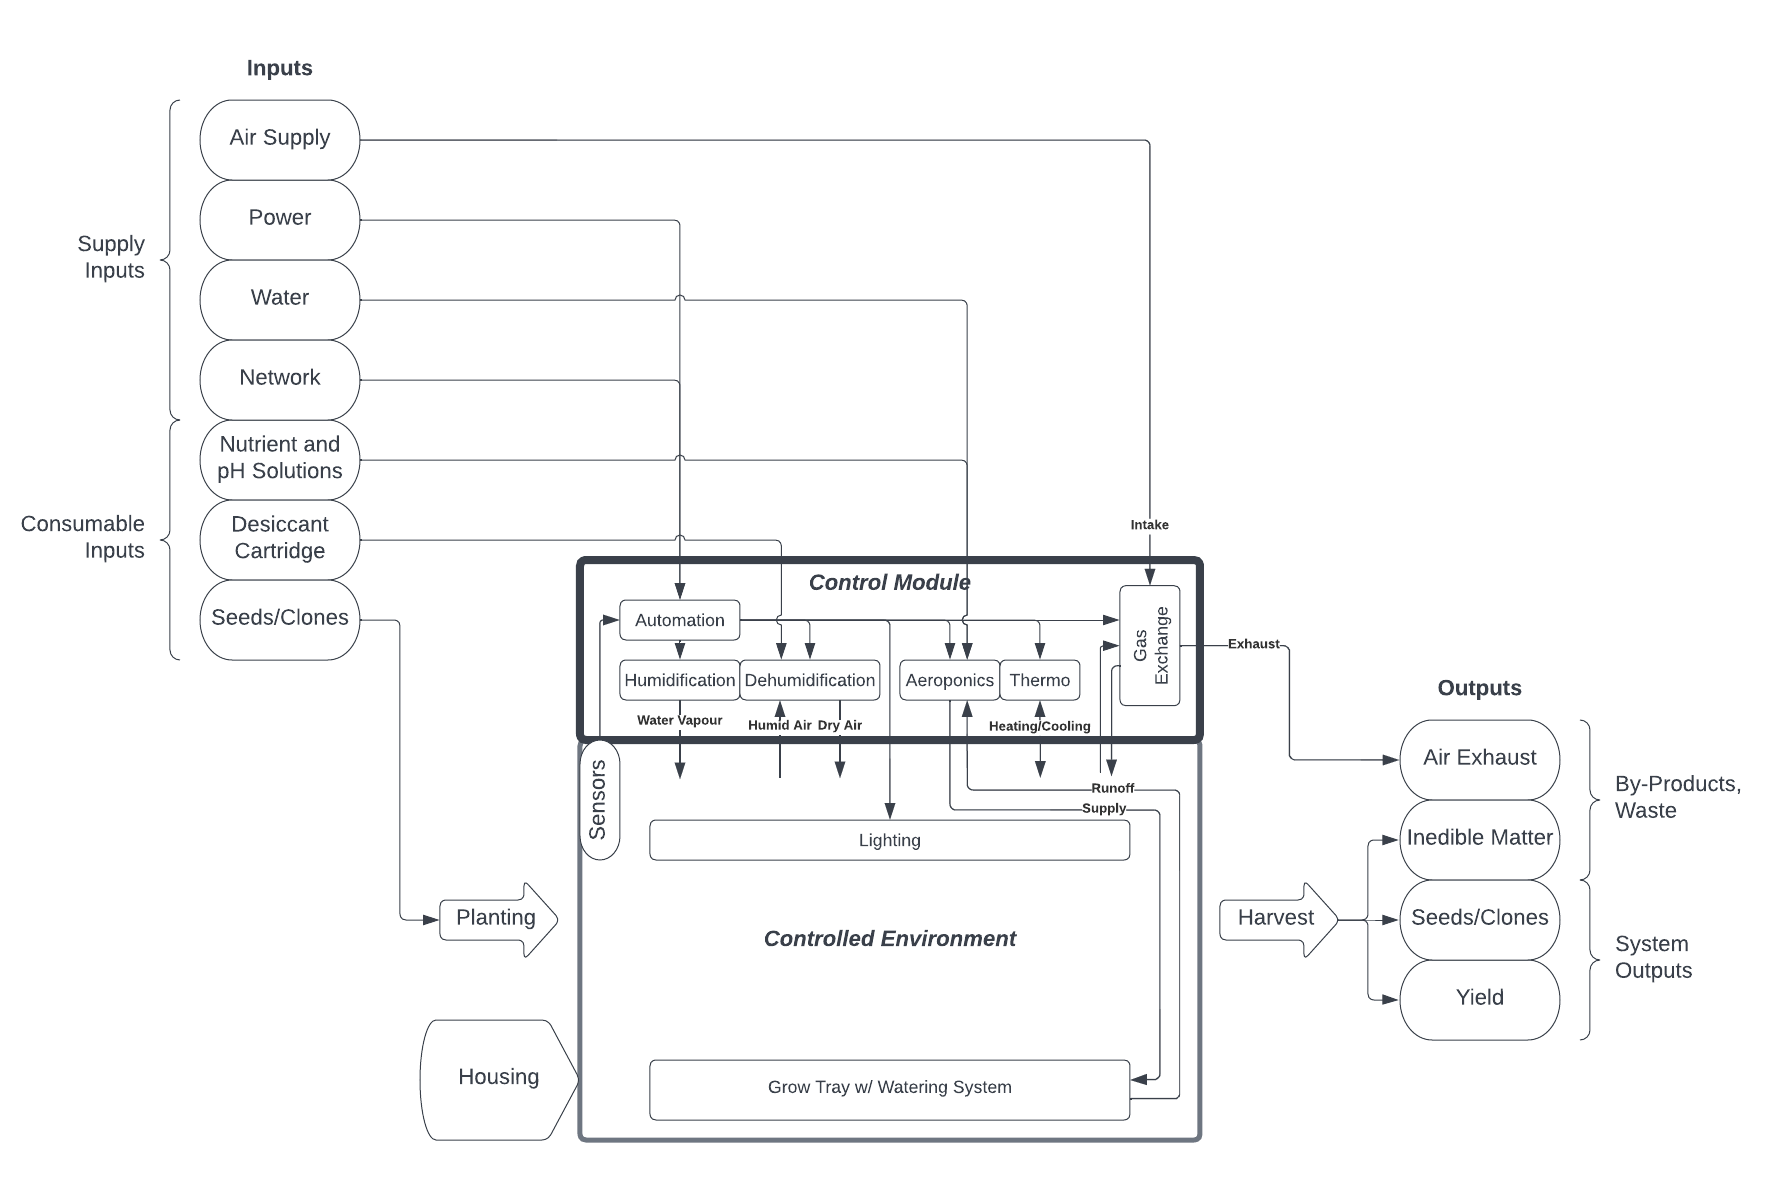
\includegraphics[width=\textwidth]{../assets/figures/system.png}}
    \caption{System overview.}
    \label{fig:system}
\end{figure}

\clearpage

\subsubsection{Hazard Analysis: Crew Contact (Harvesting, Cleaning, Maintenance)}

\begin{table}[!ht]
    \begin{tabularx}{\linewidth}{|ll|X|}
    \hline \multicolumn{2}{|l|}
        {\textbf{Source}}           & Crew contact with system during harvesting, cleaning, and maintenance  \\ \hline \multicolumn{2}{|l|}
        {\textbf{Identification}}   & Pathogens (bacteria, fungi, viruses) transferred from crew to system   \\ \hline \multicolumn{1}{|l|}{\multirow{3}{*}
        {\textbf{Evaluation}}}
        & \textit{Severity}         & Transfer of biological pathogens onto system surfaces has the potential to infect crops, posing a hazard to crew health during harvesting and ingestion. \\ \cline{2-3} \multicolumn{1}{|l|}{}
        & \textit{Likelihood}       & Fungi and viruses are of very low probability, as they cannot live on surfaces. Human gut bacteria (i.e. E. coli) is of low probability, as crew sanitation procedures are well-established. \\ \cline{2-3} \multicolumn{1}{|l|}{}
        & \textit{CCP?}             & The HACCP team determines that the risks of cross-contamination or infection are very low. Crew sanitation practices (especially prior to system interaction), practices that minimize system interaction, and sanitizing food outputs prior to consumption are adequate to control this potential hazard. \\ \hline
    \end{tabularx}
    \caption{Hazard analysis: pathogens transferred from crew to system.}
    \label{tab:hazardanalysis_systemcontact_1}
\end{table}

\begin{table}[!ht]
    \begin{tabularx}{\linewidth}{|ll|X|}
    \hline \multicolumn{2}{|l|}
        {\textbf{Source}}           & Crew contact with system during harvesting, cleaning, and maintenance \\ \hline \multicolumn{2}{|l|}
        {\textbf{Identification}}   & Pathogens (bacteria, fungi, viruses) transferred from system to crew \\ \hline \multicolumn{1}{|l|}{\multirow{3}{*}
        {\textbf{Evaluation}}}
        & \textit{Severity}         & Biological pathogens present in system materials have the potential to infect crew during interaction. \\ \cline{2-3} \multicolumn{1}{|l|}{}
        & \textit{Likelihood}       & All pathogens are of moderate probability, as they can be present in infected seeds (and thus food products at the time of ingestion). However, there are no known instances of plant-borne pathogens infecting humans. Bacteria can also be present on all surfaces. \\ \cline{2-3} \multicolumn{1}{|l|}{}
        & \textit{CCP?}             & The HACCP team determines that the risks of infection are low. However, for the sake of maximizing yield acceptability and consistency, care should be taken in seed sanitization. This, along with system sanitation practices (both pre-flight and during harvest) and practices that minimize system interaction, are adequate to control this potential hazard. \\ \hline
    \end{tabularx}
    \caption{Hazard analysis: pathogens transferred from system to crew.}
    \label{tab:hazardanalysis_systemcontact_2}
\end{table}

\clearpage

\begin{table}[!ht]
    \begin{tabularx}{\linewidth}{|ll|X|}
    \hline \multicolumn{2}{|l|}
        {\textbf{Source}}           & Crew contact with system during harvesting, cleaning, and maintenance \\ \hline \multicolumn{2}{|l|}
        {\textbf{Identification}}   & Chemical hazards to crew (i.e. heavy metals, process chemicals) introduced by system \\ \hline \multicolumn{1}{|l|}{\multirow{3}{*}
        {\textbf{Evaluation}}}
        & \textit{Severity}         & Heavy metals (i.e. lead) and chemicals introduced during manufacturing pose a threat to crew health, either during system interaction or food product ingestion. In addition, process chemicals (i.e. acidic/ basic solutions) can pose a hazard either through physical contact or accidental ingestion. \\ \cline{2-3} \multicolumn{1}{|l|}{}
        & \textit{Likelihood}       & Heavy metals are of low probability, but may be present in trace amounts in components (i.e. plumbing, electronics) and thus may come either in direct physical contact with crew(i.e. during maintenance) or be present in food products (i.e. uptake via water supply). \\ \cline{2-3} \multicolumn{1}{|l|}{}
        & \textit{CCP?}             & The HACCP team determines that the risks of heavy metal ingestion are low. All electronics, circuit boards, solder, plumbing fittings, are certified lead-free. All soldered surfaces are cleaned of flux residue. In addition, the aeroponic system is flushed of all process chemicals prior to crew interaction. Practices that include cleaning system surfaces after manufacturing, wearing gloves during handling and interaction, and cleaning food outputs of residue prior to consumption, are adequate to control this potential hazard. \\ \hline
    \end{tabularx}
    \caption{Hazard analysis: chemical hazards to system introduced by crew.}
    \label{tab:hazardanalysis_systemcontact_3}
\end{table}

\begin{table}[!ht]
    \begin{tabularx}{\linewidth}{|ll|X|}
    \hline \multicolumn{2}{|l|}
        {\textbf{Source}}           & Crew contact with system during harvesting, cleaning, and maintenance \\ \hline \multicolumn{2}{|l|}
        {\textbf{Identification}}   & Chemical hazards to system (i.e. disinfectants) introduced by crew \\ \hline \multicolumn{1}{|l|}{\multirow{3}{*}
        {\textbf{Evaluation}}}
        & \textit{Severity}         & Chemicals can remain on system surfaces, and may be present in food product, posing a hazard either through physical contact with surfaces or through ingestion. \\ \cline{2-3} \multicolumn{1}{|l|}{}
        & \textit{Likelihood}       & Disinfectants are of moderate probability. In addition, process chemicals used during maintenance (i.e. descaling agents for the aeroponics system) may be present on food product surfaces (i.e. root vegetables). \\ \cline{2-3} \multicolumn{1}{|l|}{}
        & \textit{CCP?}             & The HACCP team determines that the risks of chemical ingestion are low. Disinfectants are food-safe and dilute. In addition, the aeroponic system is flushed of all process chemicals prior to crew interaction. Practices that include wearing gloves during handling and interaction, wiping surfaces and food products with pure water prior to physical contact and ingestion, and practices that minimize system interaction are adequate to control this potential hazard. \\ \hline
    \end{tabularx}
    \caption{Hazard analysis: chemical hazards to crew introduced by system.}
    \label{tab:hazardanalysis_systemcontact_4}
\end{table}

\clearpage

\subsubsection{Hazard Analysis: Water Supply}
\begin{table}[!ht]
    \begin{tabularx}{\linewidth}{|ll|X|}
    \hline \multicolumn{2}{|l|}
        {\textbf{Source}}           & Water supply as a medium for accumulation and distribution of hazards \\ \hline \multicolumn{2}{|l|}
        {\textbf{Identification}}   & Chemical hazards (i.e. heavy metals, process chemicals) build up in water supply and transfer to produce and, in turn, crew  \\ \hline \multicolumn{1}{|l|}{\multirow{3}{*}
        {\textbf{Evaluation}}}
        & \textit{Severity}         & Heavy metals (i.e. lead) and chemicals introduced during manufacturing and process pose a threat to crew health when ingested via food product ingestion. In addition, buildup can compromise other systems (i.e. flow rate) and reduce resistance to other threats. \\ \cline{2-3} \multicolumn{1}{|l|}{}
        & \textit{Likelihood}       & Heavy metals are of low probability, but may be present in trace amounts in components (i.e. plumbing, electronics) and thus may be present in water supply for periods of time. However, regular flushing and cleansing of the supply will provide an upper bound on possible concentrations both in the supply and in any given produce. \\ \cline{2-3} \multicolumn{1}{|l|}{}
        & \textit{CCP?}             & The HACCP team determines that the risks of chemical accumulation are low. All electronics, circuit boards, solder, plumbing fittings, are certified lead-free. All soldered surfaces are cleaned of flux residue. In addition, the aeroponic system is flushed of all process chemicals prior to crew interaction. Practices that include cleaning system surfaces after manufacturing, wearing gloves during handling and interaction, and cleaning food outputs of residue prior to consumption, are adequate to control this potential hazard. \\ \hline
    \end{tabularx}
    \caption{Hazard analysis: chemical hazards accumulate in water system.}
    \label{tab:hazardanalysis_watersupply_1}
\end{table}

\begin{table}[!ht]
    \begin{tabularx}{\linewidth}{|ll|X|}
    \hline \multicolumn{2}{|l|}
        {\textbf{Source}}           & Water supply as a medium for accumulation and distribution of hazards \\ \hline \multicolumn{2}{|l|}
        {\textbf{Identification}}   & Bacteria present in water supply thrive, transfer to produce and, in turn, crew\\ \hline \multicolumn{1}{|l|}{\multirow{3}{*}
        {\textbf{Evaluation}}}
        & \textit{Severity}         & Bacteria in/on produce, surfaces, or suspended in mist can infect crew.  \\ \cline{2-3} \multicolumn{1}{|l|}{}
        & \textit{Likelihood}       & Probability of human-borne bacteria (i.e. \textit{E. coli}) is unlikely given stringent crew sanitation procedures. Other sources are infected seeds, however there are no known instances of plant-borne pathogens infecting humans. \\ \cline{2-3} \multicolumn{1}{|l|}{}
        & \textit{CCP?}             & The HACCP team determines that the risks of bacteria accumulation are low. Practices that include cleaning system surfaces after interaction, wearing gloves during handling, and flushing the water system regularly are adequate to control this potential hazard. \\ \hline
    \end{tabularx}
    \caption{Hazard analysis: bacteria grow in water system.}
    \label{tab:hazardanalysis_watersupply_2}
\end{table}

\clearpage
\subsubsection{Hazard Analysis: Nutrient Supply}
\begin{table}[!ht]
    \begin{tabularx}{\linewidth}{|ll|X|}
    \hline \multicolumn{2}{|l|}
        {\textbf{Source}}           & Nutrient Supply as a medium for accumulation and distribution of hazards \\ \hline \multicolumn{2}{|l|}
        {\textbf{Identification}}   & Bacteria in nutrient supply thrive, transfer to water and, in turn, crew  \\ \hline \multicolumn{1}{|l|}{\multirow{3}{*}
        {\textbf{Evaluation}}}
        & \textit{Severity}         & Bacteria from nutrient supply can be distributed throughout the system and infect crew. \\ \cline{2-3} \multicolumn{1}{|l|}{}
        & \textit{Likelihood}       & Nutrient supply is kept in pre-sealed packets of individual doses, meaning control on earth will eliminate introduction of threats via nutrient supply. Once in use, any bacteria will have come from the system, so presence in the nutrient supply is non-additive. \\ \cline{2-3} \multicolumn{1}{|l|}{}
        & \textit{CCP?}             & The HACCP team determines that the risks of biological threats in the nutrient supply are low. Given proper care in pre-flight steps and standard operating procedures when interacting with nutrient supply, enough practices are in place to control this hazard. \\ \hline
    \end{tabularx}
    \caption{Hazard analysis: bacteria grow in water system.}
    \label{tab:hazardanalysis_nutrientsupply_1}
\end{table}

\clearpage

\subsubsection{Hazard Analysis: Seeds}
\begin{table}[!ht]
    \begin{tabularx}{\linewidth}{|ll|X|}
    \hline \multicolumn{2}{|l|}
        {\textbf{Source}}           & Nutrient Supply as a medium for introduction of hazards \\ \hline \multicolumn{2}{|l|}
        {\textbf{Identification}}   & Pathogens (bacteria, fungi, viruses) present in seed supply are introduced to system  \\ \hline \multicolumn{1}{|l|}{\multirow{3}{*}
        {\textbf{Evaluation}}}
        & \textit{Severity}         & Minimal, there are no known occurences of plant-borne pathogens infecting humans.\\ \cline{2-3} \multicolumn{1}{|l|}{}
        & \textit{Likelihood}       & Moderate, however introduction of a pathogen will have occured pre-flight. But, they are sanitized and stored in isolated pouches which also minimize likelihood of bacteria on their surfaces.\\ \cline{2-3} \multicolumn{1}{|l|}{}
        & \textit{CCP?}             & The HACCP team determines that the risks of biological threats in the seed supply are low. Given proper care in pre-flight steps and standard operating procedures when planting seeds, enough practices are in place to control this minimally risky hazard. \\ \hline
    \end{tabularx}
    \caption{Hazard analysis: bacteria grow in water system.}
    \label{tab:hazardanalysis_nutrientsupply_1}
\end{table}


\subsection{Critical Points}

No critical points were identified in hazard analysis.
%assembly: only approved parts that have been checked for leaks, contamination, materials, air-tightness

%seeds: vetted and tested breed from an approved supplier, not opened until moment of planting, food safety steps followed while doing so (hand washing, gloves, masks, hairnet...)

%growth medium: tested for bacteria/pests, handled carefully before installation

%system inputs: filtered air, clean water, properly sourced nutrients, all tested by appropriate standards

%maintenance: plants properly isolated when non-food safe materials are present---i.e. if LED boards need to be swapped, if something needs to be greased, if something needs to be glued

%harvesting: all food safety guidelines to be followed - hand washing, gloves, masks, washing, etc.

%re-planting: checking for no old growth medium, sanitizing growth tray with food-safe sanitizer

% \subsubsection{Critical Point A}
% % Repeat for all control points

% \textbf{Hazard Description}
% % aka hazard analysis, discover CCPs

% \textbf{Critical Limits}
% % What is the safe range AND the failure conditions for the CCP

% \textbf{Monitoring Procedures}
% % How do we know the state of the CCP

% \textbf{Deviation Procedures}
% % aka corrective actions
% % How do we keep the CCP within range?

% \textbf{Associated Documents}
% record-keeping and documentation procedures

% TODO: Verification Procedures?

\subsection{Standard Test Record}
% TODO: What exactly is this?

% EXAMPLE

% Record for ingredients/materials for which critical limits have been established.
    % Supplier certification records documenting compliance of an ingredient/material with a critical limit.
    % Processor audit records verifying supplier compliance.
    % Storage records (e.g., time, temperature) for when ingredient/material storage is a CCP.

% Processing, storage and distribution records
    % Information that establishes the efficacy of a CCP to maintain product safety.
    % Data establishing the safe shelf life of the product; if age of product can affect safety.
    % Records indicating compliance with critical limits when packaging materials, labeling or sealing specifications are necessary for food safety.
    % Monitoring records.
    % Verification records.

% Deviation and corrective action records.

% Employee training records that are pertinent to CCPs and the HACCP plan.

% Documentation of the adequacy of the HACCP plan from a knowledgeable HACCP expert.

No critical points were identified in hazard analysis.

% \subsubsection{Purpose and Summary}

% \subsubsection{Safety and Quality}

% \subsubsection{Test Processes}

% \textbf{Preparation of Inputs}\\


% \textbf{Verification}\\


% \textbf{Setup, Maintenance, and Collection Protocols}\\


% \textbf{Storage}\\


% \textbf{Cleanup and Turnover}\\


% \subsubsection{Closeout}



\newpage

% References
\bibliographystyle{IEEEtran}
\bibliography{references}
\end{document}

\clearpage

\section{Hazard Analysis and Critical Control Point (HACCP) Plan}
% Specific focus on the safety of the system's processes and food outputs

% HACCP is a systematic approach to the identification, evaluation, and control of food safety hazards. A HACCP Plan is the written document which is based upon the principles of HACCP and which delineates the procedures to be followed.
% The Teams’ HACCP Plan should follow the principles and guidelines of a HACCP Plan as described by the U.S. National Advisory Committee on Microbiological Criteria for Foods (NACMCF) and the associated prerequisite programs (where applicable).
% The Basic HACCP Plan desired at this Progress Report stage (May 31 deadline) is only expected to be a starting point for the final Basic HACCP Plan expected to be a part of the final report (due in January 2023).

% Def'n of terms: https://www.fda.gov/food/hazard-analysis-critical-control-point-haccp/haccp-principles-application-guidelines#princ
% HACCP reference: https://spinoff.nasa.gov/moon-landing-food-safety?utm_source=TWITTER&utm_medium=KathyLueders&utm_campaign=NASASocial&linkId=141839394

\subsection{Food Production System Description}
% Incl. flowchart

% PeaPod uses automated control systems to generate desired environments. These are air thermoregulation, humidity control, LED lighting, and an aeroponics system. They are automated by an onboard computer and housed in a "control module" at the top of the unit. This lets power be "multiplied" for extended PeaPods by adding more control modules in a controller-follower topology.

% PeaPod is an automated plant growth environment, comprised of several control systems regulated by an automation and monitoring system within a modular, cubic housing. It can generate any desired environment while collecting data on plant growth and improving yields. Due to the wide range of actuation for each control system's environment parameter, and the extendable housing topology, the growth environment is adaptable to any plant or mission requirements. In addition, plant growth support platforms (with watering system) and lighting systems are built on modular "trays" mounted to the inside of the housing so the user can position plants and lights to accommodate any plant size.

% PeaPod's control systems are made of environmental controls (feedback loops with sensors) and plant inputs (set-states):
% \begin{itemize}
%     \item\textit{Lighting}: A wide spectrum of LEDs, from IR to UV, with a focus on Photosynthetically Active Radiation (PAR). Dimmable LED drivers enable precision spectrum and intensity control. Efficient, precise emission spectrum, low heat.
%     \item \textit{Aeroponics}: Reverse osmosis (RO) water is pressurized by a pump (with sensor for safety cutoff), brought to temperature, nutrient-dosed and pH-balanced by custom peristaltic pumps (allows for accurate dosing, and prevents backflow under pressure), and forced through nozzles to generate mist. Root zone air temperature is regulated in the same way as the leaf zone system. Exceptions include an aluminum water block (vs internal heat sink and fan) and a single temperature sensor after the block for PID feedback in a flowing system. Runoff water is recycled. Water-efficient (98\% less water use than farming), nutrient-efficient (60\% less use than farming), no pH/nutrient "feedback" loop or waste water (common in hydroponics), increased root oxygenation.
%     \item \textit{Leaf-Zone Thermoregulation}: Leaf zone air temperature is regulated by a thermoelectric heat pump. Fans blow air over heat sinks connected to either face of a Peltier tile to circulate air and dissipate heat. A Proportionate-Integral-Derivative (PID) control system is informed by temperature sensors, and controls the direction and magnitude of the heat transfer. Low complexity, high safety/reliability, easy to automate (bidirectional, precisely dimmable, PID tuning).
%     \item \textit{Humidity Regulation}: Leaf zone humidity is regulated by a dead-zone bang-bang control system informed by humidity sensors.
%     \begin{itemize}
%         \item \textit{Humidification}: RO water is supplied to a tank with a fine mesh piezoelectric disc. A controllable driver circuit oscillates the disk, producing water vapour. Easy to automate.
%         \item \textit{Dehumidification}: A dry silica gel bead cartridge is covered by servo-actuated "shutters" to control dehumidification. Fans draw humid air through a HEPA filter into the desiccant and back into the growth environment on demand. The beads change color to indicate water saturation. The crew is then notified to swap and "recharge" via evaporation in a standard oven.
%     \end{itemize}
%     \item \textit{Gas Composition Regulation and Exchange}: Oxygen and carbon dioxide levels are managed by gas exchange. Input and output ports allow fans to draw air into and out of the system. HEPA filters remove microbes and aerosols, and servo-actuated "shutters" prevent unintended exchange. Gas concentration sensors inform a bang-bang control system for port activation.
% \end{itemize}

\begin{figure}[h!]
    \centering
    \frame{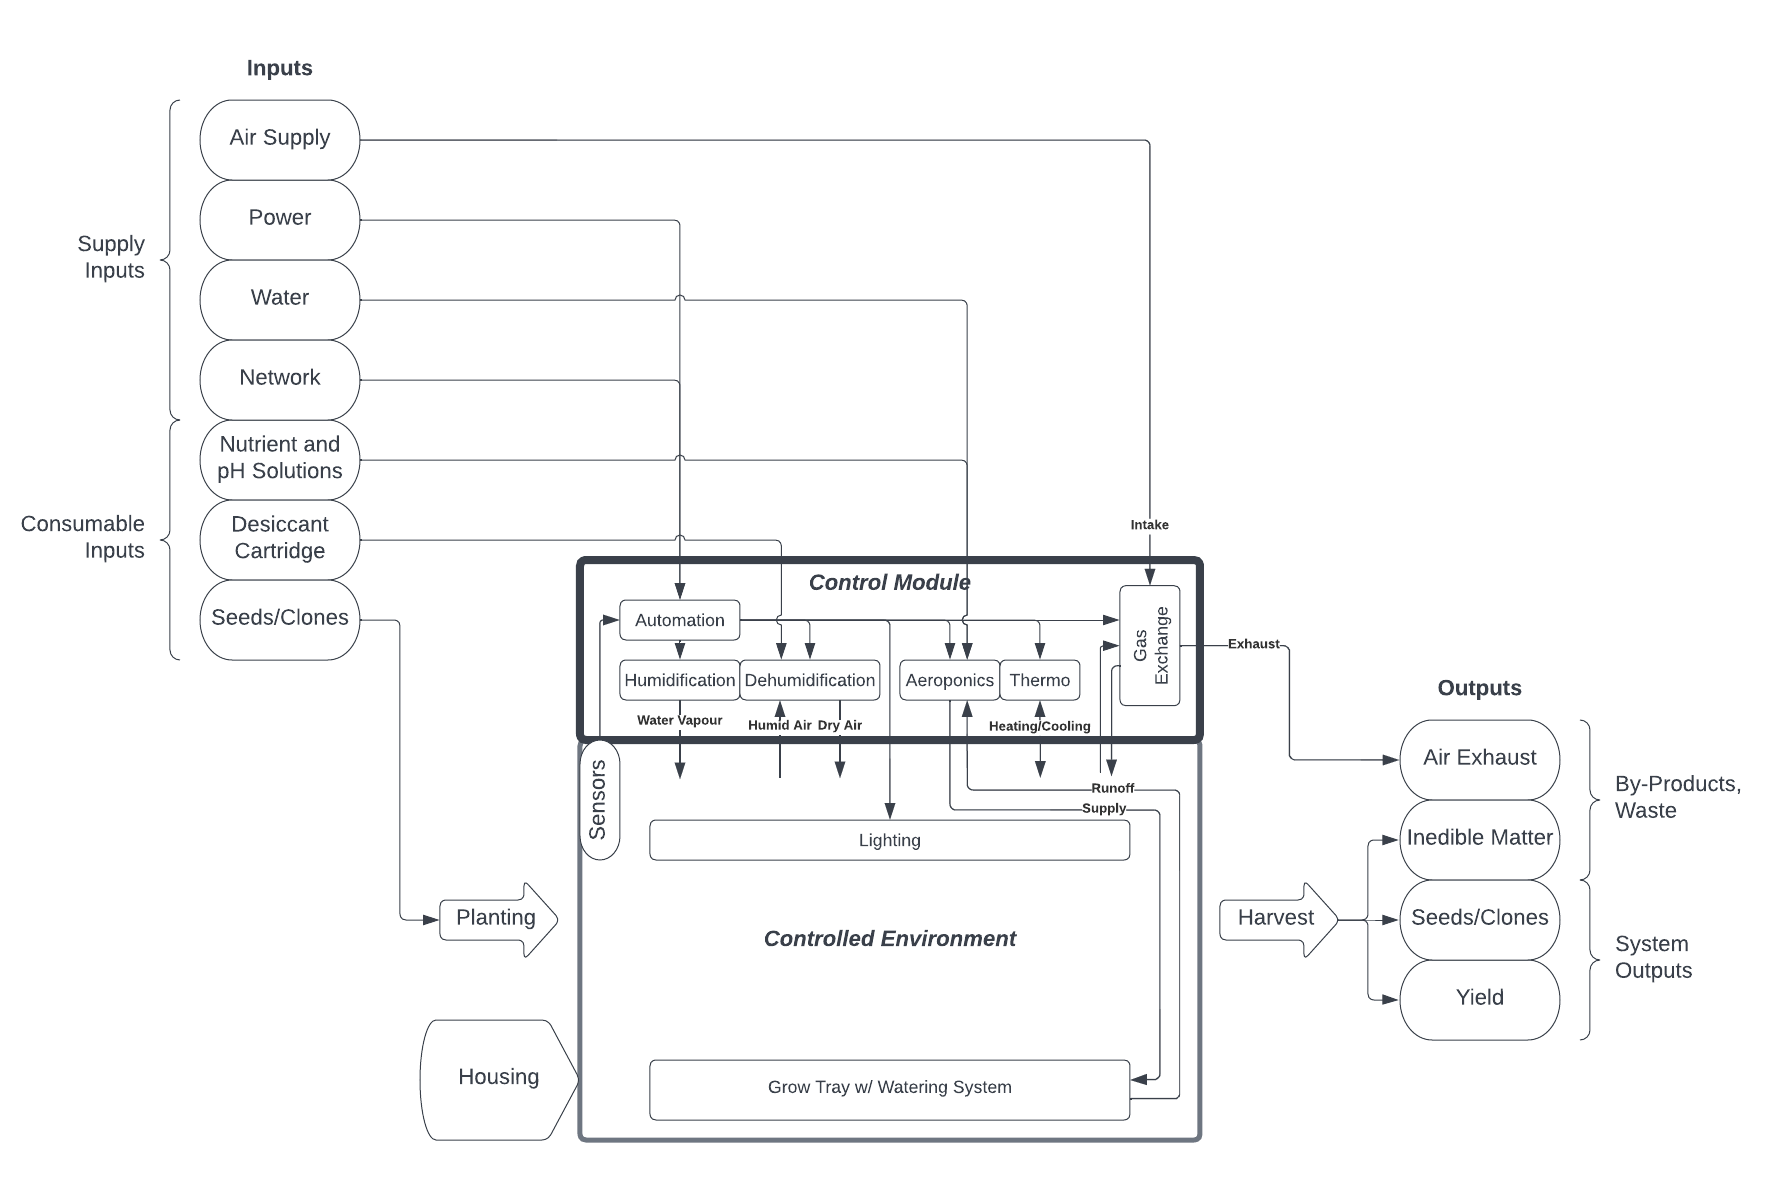
\includegraphics[width=\textwidth]{../assets/figures/system.png}}
    \caption{System overview.}
    \label{fig:system}
\end{figure}

\clearpage

\subsubsection{Hazard Analysis: Crew Contact (Harvesting, Cleaning, Maintenance)}

\begin{table}[!ht]
    \begin{tabularx}{\linewidth}{|ll|X|}
    \hline \multicolumn{2}{|l|}
        {\textbf{Source}}           & Crew contact with system during harvesting, cleaning, and maintenance  \\ \hline \multicolumn{2}{|l|}
        {\textbf{Identification}}   & Pathogens (bacteria, fungi, viruses) transferred from crew to system   \\ \hline \multicolumn{1}{|l|}{\multirow{3}{*}
        {\textbf{Evaluation}}}
        & \textit{Severity}         & Transfer of biological pathogens onto system surfaces has the potential to infect crops, posing a hazard to crew health during harvesting and ingestion. \\ \cline{2-3} \multicolumn{1}{|l|}{}
        & \textit{Likelihood}       & Fungi and viruses are of very low probability, as they cannot live on surfaces. Human gut bacteria (i.e. E. coli) is of low probability, as crew sanitation procedures are well-established. \\ \cline{2-3} \multicolumn{1}{|l|}{}
        & \textit{CCP?}             & The HACCP team determines that the risks of cross-contamination or infection are very low. Crew sanitation practices (especially prior to system interaction), practices that minimize system interaction, and sanitizing food outputs prior to consumption are adequate to control this potential hazard. \\ \hline
    \end{tabularx}
    \caption{Hazard analysis: pathogens transferred from crew to system.}
    \label{tab:hazardanalysis_systemcontact_1}
\end{table}

\begin{table}[!ht]
    \begin{tabularx}{\linewidth}{|ll|X|}
    \hline \multicolumn{2}{|l|}
        {\textbf{Source}}           & Crew contact with system during harvesting, cleaning, and maintenance \\ \hline \multicolumn{2}{|l|}
        {\textbf{Identification}}   & Pathogens (bacteria, fungi, viruses) transferred from system to crew \\ \hline \multicolumn{1}{|l|}{\multirow{3}{*}
        {\textbf{Evaluation}}}
        & \textit{Severity}         & Biological pathogens present in system materials have the potential to infect crew during interaction. \\ \cline{2-3} \multicolumn{1}{|l|}{}
        & \textit{Likelihood}       & All pathogens are of moderate probability, as they can be present in infected seeds (and thus food products at the time of ingestion). However, there are no known instances of plant-borne pathogens infecting humans. Bacteria can also be present on all surfaces. \\ \cline{2-3} \multicolumn{1}{|l|}{}
        & \textit{CCP?}             & The HACCP team determines that the risks of infection are low. However, for the sake of maximizing yield acceptability and consistency, care should be taken in seed sanitization. This, along with system sanitation practices (both pre-flight and during harvest) and practices that minimize system interaction, are adequate to control this potential hazard. \\ \hline
    \end{tabularx}
    \caption{Hazard analysis: pathogens transferred from system to crew.}
    \label{tab:hazardanalysis_systemcontact_2}
\end{table}

\clearpage

\begin{table}[!ht]
    \begin{tabularx}{\linewidth}{|ll|X|}
    \hline \multicolumn{2}{|l|}
        {\textbf{Source}}           & Crew contact with system during harvesting, cleaning, and maintenance \\ \hline \multicolumn{2}{|l|}
        {\textbf{Identification}}   & Chemical hazards to crew (i.e. heavy metals, process chemicals) introduced by system \\ \hline \multicolumn{1}{|l|}{\multirow{3}{*}
        {\textbf{Evaluation}}}
        & \textit{Severity}         & Heavy metals (i.e. lead) and chemicals introduced during manufacturing pose a threat to crew health, either during system interaction or food product ingestion. In addition, process chemicals (i.e. acidic/ basic solutions) can pose a hazard either through physical contact or accidental ingestion. \\ \cline{2-3} \multicolumn{1}{|l|}{}
        & \textit{Likelihood}       & Heavy metals are of low probability, but may be present in trace amounts in components (i.e. plumbing, electronics) and thus may come either in direct physical contact with crew(i.e. during maintenance) or be present in food products (i.e. uptake via water supply). \\ \cline{2-3} \multicolumn{1}{|l|}{}
        & \textit{CCP?}             & The HACCP team determines that the risks of heavy metal ingestion are low. All electronics, circuit boards, solder, plumbing fittings, are certified lead-free. All soldered surfaces are cleaned of flux residue. In addition, the aeroponic system is flushed of all process chemicals prior to crew interaction. Practices that include cleaning system surfaces after manufacturing, wearing gloves during handling and interaction, and cleaning food outputs of residue prior to consumption, are adequate to control this potential hazard. \\ \hline
    \end{tabularx}
    \caption{Hazard analysis: chemical hazards to system introduced by crew.}
    \label{tab:hazardanalysis_systemcontact_3}
\end{table}

\begin{table}[!ht]
    \begin{tabularx}{\linewidth}{|ll|X|}
    \hline \multicolumn{2}{|l|}
        {\textbf{Source}}           & Crew contact with system during harvesting, cleaning, and maintenance \\ \hline \multicolumn{2}{|l|}
        {\textbf{Identification}}   & Chemical hazards to system (i.e. disinfectants) introduced by crew \\ \hline \multicolumn{1}{|l|}{\multirow{3}{*}
        {\textbf{Evaluation}}}
        & \textit{Severity}         & Chemicals can remain on system surfaces, and may be present in food product, posing a hazard either through physical contact with surfaces or through ingestion. \\ \cline{2-3} \multicolumn{1}{|l|}{}
        & \textit{Likelihood}       & Disinfectants are of moderate probability. In addition, process chemicals used during maintenance (i.e. descaling agents for the aeroponics system) may be present on food product surfaces (i.e. root vegetables). \\ \cline{2-3} \multicolumn{1}{|l|}{}
        & \textit{CCP?}             & The HACCP team determines that the risks of chemical ingestion are low. Disinfectants are food-safe and dilute. In addition, the aeroponic system is flushed of all process chemicals prior to crew interaction. Practices that include wearing gloves during handling and interaction, wiping surfaces and food products with pure water prior to physical contact and ingestion, and practices that minimize system interaction are adequate to control this potential hazard. \\ \hline
    \end{tabularx}
    \caption{Hazard analysis: chemical hazards to crew introduced by system.}
    \label{tab:hazardanalysis_systemcontact_4}
\end{table}

\clearpage

\subsubsection{Hazard Analysis: Water Supply}
\begin{table}[!ht]
    \begin{tabularx}{\linewidth}{|ll|X|}
    \hline \multicolumn{2}{|l|}
        {\textbf{Source}}           & Water supply as a medium for accumulation and distribution of hazards \\ \hline \multicolumn{2}{|l|}
        {\textbf{Identification}}   & Chemical hazards (i.e. heavy metals, process chemicals) build up in water supply and transfer to produce and, in turn, crew  \\ \hline \multicolumn{1}{|l|}{\multirow{3}{*}
        {\textbf{Evaluation}}}
        & \textit{Severity}         & Heavy metals (i.e. lead) and chemicals introduced during manufacturing and process pose a threat to crew health when ingested via food product ingestion. In addition, buildup can compromise other systems (i.e. flow rate) and reduce resistance to other threats. \\ \cline{2-3} \multicolumn{1}{|l|}{}
        & \textit{Likelihood}       & Heavy metals are of low probability, but may be present in trace amounts in components (i.e. plumbing, electronics) and thus may be present in water supply for periods of time. However, regular flushing and cleansing of the supply will provide an upper bound on possible concentrations both in the supply and in any given produce. \\ \cline{2-3} \multicolumn{1}{|l|}{}
        & \textit{CCP?}             & The HACCP team determines that the risks of chemical accumulation are low. All electronics, circuit boards, solder, plumbing fittings, are certified lead-free. All soldered surfaces are cleaned of flux residue. In addition, the aeroponic system is flushed of all process chemicals prior to crew interaction. Practices that include cleaning system surfaces after manufacturing, wearing gloves during handling and interaction, and cleaning food outputs of residue prior to consumption, are adequate to control this potential hazard. \\ \hline
    \end{tabularx}
    \caption{Hazard analysis: chemical hazards accumulate in water system.}
    \label{tab:hazardanalysis_watersupply_1}
\end{table}

\begin{table}[!ht]
    \begin{tabularx}{\linewidth}{|ll|X|}
    \hline \multicolumn{2}{|l|}
        {\textbf{Source}}           & Water supply as a medium for accumulation and distribution of hazards \\ \hline \multicolumn{2}{|l|}
        {\textbf{Identification}}   & Bacteria present in water supply thrive, transfer to produce and, in turn, crew\\ \hline \multicolumn{1}{|l|}{\multirow{3}{*}
        {\textbf{Evaluation}}}
        & \textit{Severity}         & Bacteria in/on produce, surfaces, or suspended in mist can infect crew.  \\ \cline{2-3} \multicolumn{1}{|l|}{}
        & \textit{Likelihood}       & Probability of human-borne bacteria (i.e. \textit{E. coli}) is unlikely given stringent crew sanitation procedures. Other sources are infected seeds, however there are no known instances of plant-borne pathogens infecting humans. \\ \cline{2-3} \multicolumn{1}{|l|}{}
        & \textit{CCP?}             & The HACCP team determines that the risks of bacteria accumulation are low. Practices that include cleaning system surfaces after interaction, wearing gloves during handling, and flushing the water system regularly are adequate to control this potential hazard. \\ \hline
    \end{tabularx}
    \caption{Hazard analysis: bacteria grow in water system.}
    \label{tab:hazardanalysis_watersupply_2}
\end{table}

\clearpage
\subsubsection{Hazard Analysis: Nutrient Supply}
\begin{table}[!ht]
    \begin{tabularx}{\linewidth}{|ll|X|}
    \hline \multicolumn{2}{|l|}
        {\textbf{Source}}           & Nutrient Supply as a medium for accumulation and distribution of hazards \\ \hline \multicolumn{2}{|l|}
        {\textbf{Identification}}   & Bacteria in nutrient supply thrive, transfer to water and, in turn, crew  \\ \hline \multicolumn{1}{|l|}{\multirow{3}{*}
        {\textbf{Evaluation}}}
        & \textit{Severity}         & Bacteria from nutrient supply can be distributed throughout the system and infect crew. \\ \cline{2-3} \multicolumn{1}{|l|}{}
        & \textit{Likelihood}       & Nutrient supply is kept in pre-sealed packets of individual doses, meaning control on earth will eliminate introduction of threats via nutrient supply. Once in use, any bacteria will have come from the system, so presence in the nutrient supply is non-additive. \\ \cline{2-3} \multicolumn{1}{|l|}{}
        & \textit{CCP?}             & The HACCP team determines that the risks of biological threats in the nutrient supply are low. Given proper care in pre-flight steps and standard operating procedures when interacting with nutrient supply, enough practices are in place to control this hazard. \\ \hline
    \end{tabularx}
    \caption{Hazard analysis: bacteria grow in water system.}
    \label{tab:hazardanalysis_nutrientsupply_1}
\end{table}

\clearpage

\subsubsection{Hazard Analysis: Seeds}
\begin{table}[!ht]
    \begin{tabularx}{\linewidth}{|ll|X|}
    \hline \multicolumn{2}{|l|}
        {\textbf{Source}}           & Nutrient Supply as a medium for introduction of hazards \\ \hline \multicolumn{2}{|l|}
        {\textbf{Identification}}   & Pathogens (bacteria, fungi, viruses) present in seed supply are introduced to system  \\ \hline \multicolumn{1}{|l|}{\multirow{3}{*}
        {\textbf{Evaluation}}}
        & \textit{Severity}         & Minimal, there are no known occurences of plant-borne pathogens infecting humans.\\ \cline{2-3} \multicolumn{1}{|l|}{}
        & \textit{Likelihood}       & Moderate, however introduction of a pathogen will have occured pre-flight. But, they are sanitized and stored in isolated pouches which also minimize likelihood of bacteria on their surfaces.\\ \cline{2-3} \multicolumn{1}{|l|}{}
        & \textit{CCP?}             & The HACCP team determines that the risks of biological threats in the seed supply are low. Given proper care in pre-flight steps and standard operating procedures when planting seeds, enough practices are in place to control this minimally risky hazard. \\ \hline
    \end{tabularx}
    \caption{Hazard analysis: bacteria grow in water system.}
    \label{tab:hazardanalysis_nutrientsupply_1}
\end{table}


\subsection{Critical Points}

No critical points were identified in hazard analysis.
%assembly: only approved parts that have been checked for leaks, contamination, materials, air-tightness

%seeds: vetted and tested breed from an approved supplier, not opened until moment of planting, food safety steps followed while doing so (hand washing, gloves, masks, hairnet...)

%growth medium: tested for bacteria/pests, handled carefully before installation

%system inputs: filtered air, clean water, properly sourced nutrients, all tested by appropriate standards

%maintenance: plants properly isolated when non-food safe materials are present---i.e. if LED boards need to be swapped, if something needs to be greased, if something needs to be glued

%harvesting: all food safety guidelines to be followed - hand washing, gloves, masks, washing, etc.

%re-planting: checking for no old growth medium, sanitizing growth tray with food-safe sanitizer

% \subsubsection{Critical Point A}
% % Repeat for all control points

% \textbf{Hazard Description}
% % aka hazard analysis, discover CCPs

% \textbf{Critical Limits}
% % What is the safe range AND the failure conditions for the CCP

% \textbf{Monitoring Procedures}
% % How do we know the state of the CCP

% \textbf{Deviation Procedures}
% % aka corrective actions
% % How do we keep the CCP within range?

% \textbf{Associated Documents}
% record-keeping and documentation procedures

% TODO: Verification Procedures?

\subsection{Standard Test Record}
% TODO: What exactly is this?

% EXAMPLE

% Record for ingredients/materials for which critical limits have been established.
    % Supplier certification records documenting compliance of an ingredient/material with a critical limit.
    % Processor audit records verifying supplier compliance.
    % Storage records (e.g., time, temperature) for when ingredient/material storage is a CCP.

% Processing, storage and distribution records
    % Information that establishes the efficacy of a CCP to maintain product safety.
    % Data establishing the safe shelf life of the product; if age of product can affect safety.
    % Records indicating compliance with critical limits when packaging materials, labeling or sealing specifications are necessary for food safety.
    % Monitoring records.
    % Verification records.

% Deviation and corrective action records.

% Employee training records that are pertinent to CCPs and the HACCP plan.

% Documentation of the adequacy of the HACCP plan from a knowledgeable HACCP expert.

No critical points were identified in hazard analysis.

% \subsubsection{Purpose and Summary}

% \subsubsection{Safety and Quality}

% \subsubsection{Test Processes}

% \textbf{Preparation of Inputs}\\


% \textbf{Verification}\\


% \textbf{Setup, Maintenance, and Collection Protocols}\\


% \textbf{Storage}\\


% \textbf{Cleanup and Turnover}\\


% \subsubsection{Closeout}



% \subsection{Materials}
\subsubsection{System}

\textbf{Automation}\\

\begin{table}[!h]
    \centering
    \begin{tabular}{|c|l|l|l|c|}
    \hline
        Index   & Manufacturer Part Number  & Manufacturer Name         & Description                       & Quantity  \\ \hline
        1       & A000005                   & Arduino                   & ARDUINO NANO ATMEGA328 EVAL BRD   & 1         \\ \hline
        2       & S404GSEJ6-U3000-3         & Delkin Devices, Inc.      & 4GB MLC MICROSD CARD (-25C - +85  & 1         \\ \hline
        3       & 61304021121               & Würth Elektronik          & CONN HEADER VERT 40POS 2.54MM     & 1         \\ \hline
        4       & SC0510                    & Raspberry Pi              & ZERO 2 W                          & 1         \\ \hline
        5       & DMN2005K-7                & Diodes Incorporated       & MOSFET N-CH 20V 300MA SOT23-3     & 2         \\ \hline
        6       & RC0603FR-0710KL           & YAGEO                     & RES 10K OHM 1\% 1/10W 0603        & 5         \\ \hline
        7       & 4484                      & Adafruit Industries LLC   & MINI PITFT 1.3 FOR RASPBERRY PI   & 1         \\ \hline
        8       & 5055670271                & Molex                     & CONN HEADER SMD R/A 2POS 1.25MM   & 2         \\ \hline
        9       & 5055670471                & Molex                     & CONN HEADER SMD R/A 4POS 1.25MM   & 5         \\ \hline
        10      & 5055670871                & Molex                     & CONN HEADER SMD R/A 8POS 1.25MM   & 3         \\ \hline
        11      & 5055670681                & Molex                     & CONN HEADER SMD R/A 6POS 1.25MM   & 3         \\ \hline
    \end{tabular}
    \caption{Automation system electronic components.}
    \label{tab:automation_components}
\end{table}

In addition, 1x \textit{Automation Motherboard PCB}: 2 Layers, 1 oz. Copper, 1.6mm Thickness, Suggested: HASL Finish (Lead-Free), White PCB, Black Silkscreen

\textbf{Housing}\\

\begin{table}[!ht]
    \centering
    \begin{tabular}{|l|l|c|l|l|}
    \hline
        Part                    & Description                                           & Quantity  & Supplier          & Supplier Part Number  \\ \hline
        Control Module Housing  & 5-Sided enclosure                                     & 1         & Protocase         & ~                     \\ \hline
        Frame Front X Extrusion & Silver Painted, 20x20mm, Ordered 2ft., Cut to 500mm   & 2         & McMaster-Carr     & 5537T101              \\ \hline
        Frame Door Y Extrusion  & Silver Painted, 20x20mm, Ordered 2ft., Cut to 500mm   & 2         & McMaster-Carr     & 5537T101              \\ \hline
        Frame Rear X Extrusion  & Silver Painted, 20x20mm, Ordered 2ft., Cut to 460mm   & 2         & McMaster-Carr     & 5537T101              \\ \hline
        Frame Door X Extrusion  & Silver Painted, 20x20mm, Ordered 2ft., Cut to 460mm   & 2         & McMaster-Carr     & 5537T101              \\ \hline
        Frame Rear Y Extrusion  & Silver Painted, 20x40mm, Ordered 2ft., Cut to 460mm   & 2         & McMaster-Carr     & 5537T111              \\ \hline
        Frame Front Y           & Silver Painted, 20x20mm, Ordered 2ft., Cut to 460mm   & 2         & McMaster-Carr     & 5537T101              \\ \hline
        Frame Z                 & Silver Painted, 20x20mm, Ordered 2ft., Cut to 460mm   & 4         & McMaster-Carr     & 5537T101              \\ \hline
        Tray X Extrusion        & Silver Painted, 20x20mm, Ordered 2ft., Cut to 440mm   & 4         & McMaster-Carr     & 5537T101              \\ \hline
        Tray Z Extrusion        & Silver Painted, 20x20mm, Ordered 2ft., Cut to 400mm   & 6         & McMaster-Carr     & 5537T101              \\ \hline
        Nozzle Arm Extrusion    & Silver Painted, 20x20mm, Ordered 1ft., Cut to 150mm   & 2         & McMaster-Carr     & 5537T101              \\ \hline
        M5x0.8 10mm Bolts       & Alloy Steel, Black Oxide Coated, Socket Head Cap      & 139       & McMaster-Carr     & 91290A224             \\ \hline
        M5x0.8 16mm Bolts       & Alloy Steel, Black Oxide Coated, Socket Head Cap      & 10        & McMaster-Carr     & 91290A232             \\ \hline
        M4x0.7 16mm Bolts       & Alloy Steel, Black Oxide Coated, Socket Head Cap      & 12        & McMaster-Carr     & 91290A154             \\ \hline
        M4x0.7 Hex Nuts         & High-Strength Steel, Black Oxide Coated               & 12        & McMaster-Carr     & 94166A110             \\ \hline
        M5 T-Nuts               & Zinc-Plated Steel, Black Painted, for 5mm Slot        & 139       & McMaster-Carr     & 5537T651              \\ \hline
        M5x0.8 Hex Nuts         & Alloy Steel, Black Oxide Coated                       & 10        & McMaster-Carr     & 94166A120             \\ \hline
        Foam Insulation         & DUROSPAN GPS R5 4ft. x 8ft. x 1in.                    & 1         & Home Depot Canada & 1001211234            \\ \hline
        Reflective Mylar        & 27in. x 12ft. x 0.002in., Aluminum-coated PET         & 1         & McMaster-Carr     & 7538T11               \\ \hline
        Adhesive                & LePage PL300 Foamboard 295mL                          & 2         & Home Depot Canada & 1000403469            \\ \hline
        Grow Cup                & 2in. Diameter                                         & 16        & Amazon            & ~                     \\ \hline
        Door Hinges             & Plastic, Black, for 20x20mm Extrusion                 & 2         & McMaster-Carr     & 5537T85               \\ \hline
        Feet Bumpers            & Adhesive-Back, Medium-Hard Polyurethane, Black        & 4         & McMaster-Carr     & 95495K24              \\ \hline
    \end{tabular}
    \caption{Housing subsystem components.}
    \label{tab:housing_parts}
\end{table}

\begin{table}[!ht]
    \centering
    \begin{tabular}{|l|c|l|l|}
    \hline
        Part                        & Quantity  & Materials             & Process           \\ \hline
        L Bracket                   & 12        & PETG Filament         & 3D Printing       \\ \hline
        L Bracket (Grow Tray)       & 4         & PETG Filament         & 3D Printing       \\ \hline
        Diagonal Bracket            & 4         & PETG Filament         & 3D Printing       \\ \hline
        T Bracket                   & 10        & PETG Filament         & 3D Printing       \\ \hline
        Tray Hook BL                & 2         & PETG Filament         & 3D Printing       \\ \hline
        Tray Hook BR                & 2         & PETG Filament         & 3D Printing       \\ \hline
        Tray Hook FL                & 2         & PETG Filament         & 3D Printing       \\ \hline
        Tray Hook FR                & 2         & PETG Filament         & 3D Printing       \\ \hline
        Grow Plate Quarters         & 4         & 210x210x5mm PET Sheet & Table Saw         \\ \hline
        Grow Plate Washer           & 1         & PETG Filament         & 3D Printing       \\ \hline
        Nozzle Mount A              & 2         & PETG Filament         & 3D Printing       \\ \hline
        Nozzle Mount B              & 2         & PETG Filament         & 3D Printing       \\ \hline
        Lighting LED Board Mount    & 5         & PETG Filament         & 3D Printing       \\ \hline
        Lighting Power Board Mount  & 1         & PETG Filament         & 3D Printing       \\ \hline
        Feet                        & 4         & PETG Filament         & 3D Printing       \\ \hline
    \end{tabular}
    \caption{Housing subsystem fabricated parts.}
    \label{tab:housing_fabrication}
\end{table}

\textbf{Aeroponics}\\


\textbf{Leaf-Zone Thermoregulation}\\


\textbf{Humidification}\\


\textbf{Dehumidification}\\


\textbf{Gas Composition Regulation and Exchange}\\


\textbf{Lighting}\\


\subsubsection{Inputs}
% Supply inputs (water, power, network), consumable inputs (pH/nutrient solutions, dehumidification cartridge)

\textbf{Supply Inputs}
\begin{itemize}
    \item \textit{Water}: reverse-osmosis, ambient
    \item \textit{Power}: 120V 60Hz AC\footnote{The power supply can be altered to suit a variety of power inputs (i.e. DC)}
    \item \textit{Network}: ethernet or wireless, optional
\end{itemize}

\textbf{Consumable Inputs}
\begin{itemize}
    \item \textit{Nutrient/pH Adjusment Solutions}: pouches
    \item \textit{Dehumidification Cartridge}: recharged
\end{itemize}

\subsubsection{Outputs}
% Food outputs(?), by-products/waste (waste water from flushing, dehumidification cartridge)

\textbf{Food Outputs}\\


\textbf{By-Products \& Waste}\\


\subsubsection{Maintenance}

\textbf{Spare Components}\\


\textbf{Tools}\\


\subsubsection{Cleaning}

\textbf{Soaps}\\


\textbf{Disinfectants}\\


\textbf{Tools}\\



% Please outline any operational risks for the technology, and your potential mitigation strategy. (limit 4000 characters)
% More specifically, please outline the following environmental & process safety requirements:
% Avoidance of hazardous compounds or materials used or produced (e.g., microbes, off-gassing, toxic components)
% Avoidance of hazards associated with cleaning this technology prior to and/or after use
% Avoidance of physical, chemical, or biological hazards associated with the hardware or the process
% Clear mitigation strategies to address the aforementioned risks

\section{Inputs and Outputs}

\subsection{Inputs}
% With a focus on the progress or changes made during Phase 2 of the challenge, please describe the inputs and their amounts needed for your food production technology (limit 6000 characters).

% Inputs could include:
% Chemicals (e.g., nutrients, acid, base, disinfection)
% Water (RO, tap etc.)
% Energy
% Cleaning supplies
% CO2 or other gases
% Other materials that enter the system
% NOTE: Unlike in Phase 1, it is no longer acceptable to estimate the quantities of your inputs based on reasonable literature values. Instead, Teams must provide data generated from direct measurement of their system, or calculations based on known system metrics (i.e. the basis for calculations must be gathered from the prototype itself, and not hypothetical).

\textit{Infrastructural Inputs}: Reverse osmosis water (constant supply at positive pressure from onboard RODI system), nutrient solutions (stored, one container each plus refill tanks), pH solutions (one container pH up, one container pH down, plus refill tanks, stored), power (onboard power, standard 120V AC 60Hz), network connection (onboard network, for remote control, live video/data transmission), plant seeds (stored in vacuum-sealed seed bank, selected for variety and acceptability), input air (HEPA filtered, carbon dioxide-rich)

\textit{Process Inputs}: Plant species identifiers, environment program (for entire growth cycle, one per plant species), nutrient and pH-adjustment solution identifiers (compounds and molarities, i.e. solution A is 0.6M NaNO${}_3$)

Common nutrient solutions target specific ions, including bioavailable nonmetals (nitrates/nitrites, ammonia/ammonium, phosphates, sulphates), metals (potassium, calcium, magnesium, iron) and other trace elements.

% With a focus on the progress made during Phase 2 of the challenge, describe the outputs of your food production technology system. (limit 3000 Characters)

% Outputs could include:
% Food products
% Waste (wastewater, inedible biomass, cleaning wipes, testing material etc.)
% Heat (latent and sensible)
% Other useable or unusable product exiting the system, including liquid and gaseous process flows (e.g., water vapor, low-molecular weight organic and inorganic compounds, water, oils, etc.)

\textit{Products}: Edible plant matter, recorded environment data, plant metric data, live video feed, time-lapse capture

\textit{Byproducts}: Inedible plant matter (stems/roots/leaves/etc., waste), sensible heat (from thermoregulation pumping, managed by onboard heating/cooling), exhaust air (via HEPA filter, sterilized and dehumidified by onboard life support, oxygen-rich), minimal water vapour (as a result of higher air humidity, minimized by housing seal), latent heat (as a result of higher leaf zone temperature, minimized by insulation)

% With a focus on the progress made during Phase 2 of the challenge, please outline the net water consumption of your food production technology (limit 4000 characters).

\textit{Humidification}: By using a mesh nebulizer to produce smaller and more consistent vapour, greater overall water consumption efficiency was achieved.

\textit{Aeroponics}: Aeroponics by design uses far less water than traditional farming. In addition, higher quality nozzles with adjustable directionality allow for more of the water to be sprayed directly at the root zone and with better and more consistent droplet sizes for better uptake. Finally, by enclosing the root zone in a watertight container, no water escapes, and runoff water collected at the bottom of the container can be recycled. 5mL/sec/nozzle @80PSI x 2 nozzles per unit x 12 units x 10 seconds misting per hour

In calculation, it is assumed that all aeroponic water is consumed, as all runoff water is recycled.

% Note: As your team’s net water consumption is previously captured, you may copy and paste your response from the constraint section above.

% With a focus on the progress or changes made during Phase 2 of the challenge, describe how the food production technology achieves the greatest amount of food output in relation to the quantity of inputs and quantity of waste output (limit 4000 characters)

\subsection{Optimization}
\label{sec:optimization}

\textbf{Purpose}: Iteratively improve yield, etc. of crops as more environment condition and plant metric data is gathered across different programs over multiple growth cycles.

\textbf{Function}:
\begin{itemize}
    \item \textbf{Inputs}: Growth cycle datasets (Environment data across time (control system portion of $\vec E(t)$), plant performance metric (PPM) data across time ($\vec P(t)$), associated program (actuated portion of $\vec E(t)$))
    \item \textbf{Outputs}: Plant-program performance prediction model, novel programs
\end{itemize}

\textbf{Method}: 

Assume a plant's growth rate (or state change) is related to its current internal state $\vec P \in \R^n$ (for $n$ plant metrics) and the environment conditions $\vec E \in \R^m$ (for $m$ environment parameters). Let these both be functions $\vec P (t),\vec E(t)$ defined at each $t$, where $t=0$ indicates the time of planting. Assume that this relationship is constant for all members of a given species.

Define plant state change $\vec P'$: 

$$\vec P'(t) = \frac{d}{dt}\vec P(t)$$

Define the plant-environment behaviour function $Q$: 

$$Q(\vec P(t), \vec E(t), t)=\vec P'(t)$$ 

Given the current internal and external states, determine the plant's state change.

\begin{enumerate}
    \item Set $\vec E_{set}(t)~\forall~ t$, aka the program (\ref{sec:automation});
    \item Record $\vec P(t)~\forall~ t$ and $\vec E(t)\approx \vec E_{set}(t)~\forall~ t$;
    \item Calculate $\vec P'(t)~\forall~ t$;
    \item Fit $\vec Q$ to our data;
\end{enumerate}

By fitting $\vec Q$ across iterations, we can predict $\vec P$ at any $\vec E$ and $t$. For example:

$$\vec P(t+\Delta t)=P(t)+\Delta t\cdot Q(\vec P(t),\vec E(t))$$

Gradient ascent with this model can be used to generate novel (theoretically improved) programs.

\textbf{Features}:
\begin{itemize}
    \item \textit{Machine Learning Model}: Represented by $Q$. Operates in the cloud.
    \item \textit{Environment Data} (over time): Represented by $\vec E(t)$. Collected by sensors (for \textit{control loop} environment parameters) and extracted from the associated program (for \textit{actuated instruction} environment parameters). See Section \ref{sec:automation}.
    \item \textit{PPM Data} (over time): Represented by $\vec P(t)$. Extracted from computer vision. See Section \ref{sec:automation}.
\end{itemize}

\section{Reliability and Stability}
% Reliability: Operational cycle time (i.e., amount of time for one production cycle) (limit 2000 characters)

% Reliability: System lifespan (i.e., how many cycles can the system perform before requiring replacement parts?) (limit 2000 characters)

% Reliability: Overview of maintenance/repair as well as cleaning processes and procedures, including (but not limited to): (limit 8000 characters)
% What the processes and procedures look like
% Maintenance schedule (i.e., how often will it need maintenance and/or cleaned?)
% Which component(s)/element(s) require cleaning 
% Amount of time required to perform the system cleaning and maintenance
% What is needed to fully clean the system (e.g., water, chemicals)
% Which component(s)/element(s) require maintenance or replacement (i.e., what components will need to be replaced, and when?)
% Critical spare parts for a three-year mission and longevity of those spare parts
% Estimated additional mass needed for replacement parts and cleaning materials
% Estimated total time needed per month, per 6 months, and per year for maintenance and cleaning

\subsection{Process Description}
\label{sec:process}
% Please give a brief update of your food production system’s process (including maintenance and cleaning):
% Fully-detailed process description (incl. setup, operation, maintenance, and cleaning), flow diagram for each
% maximum 5000 characters

\begin{figure}[h!]
    \centering
    \frame{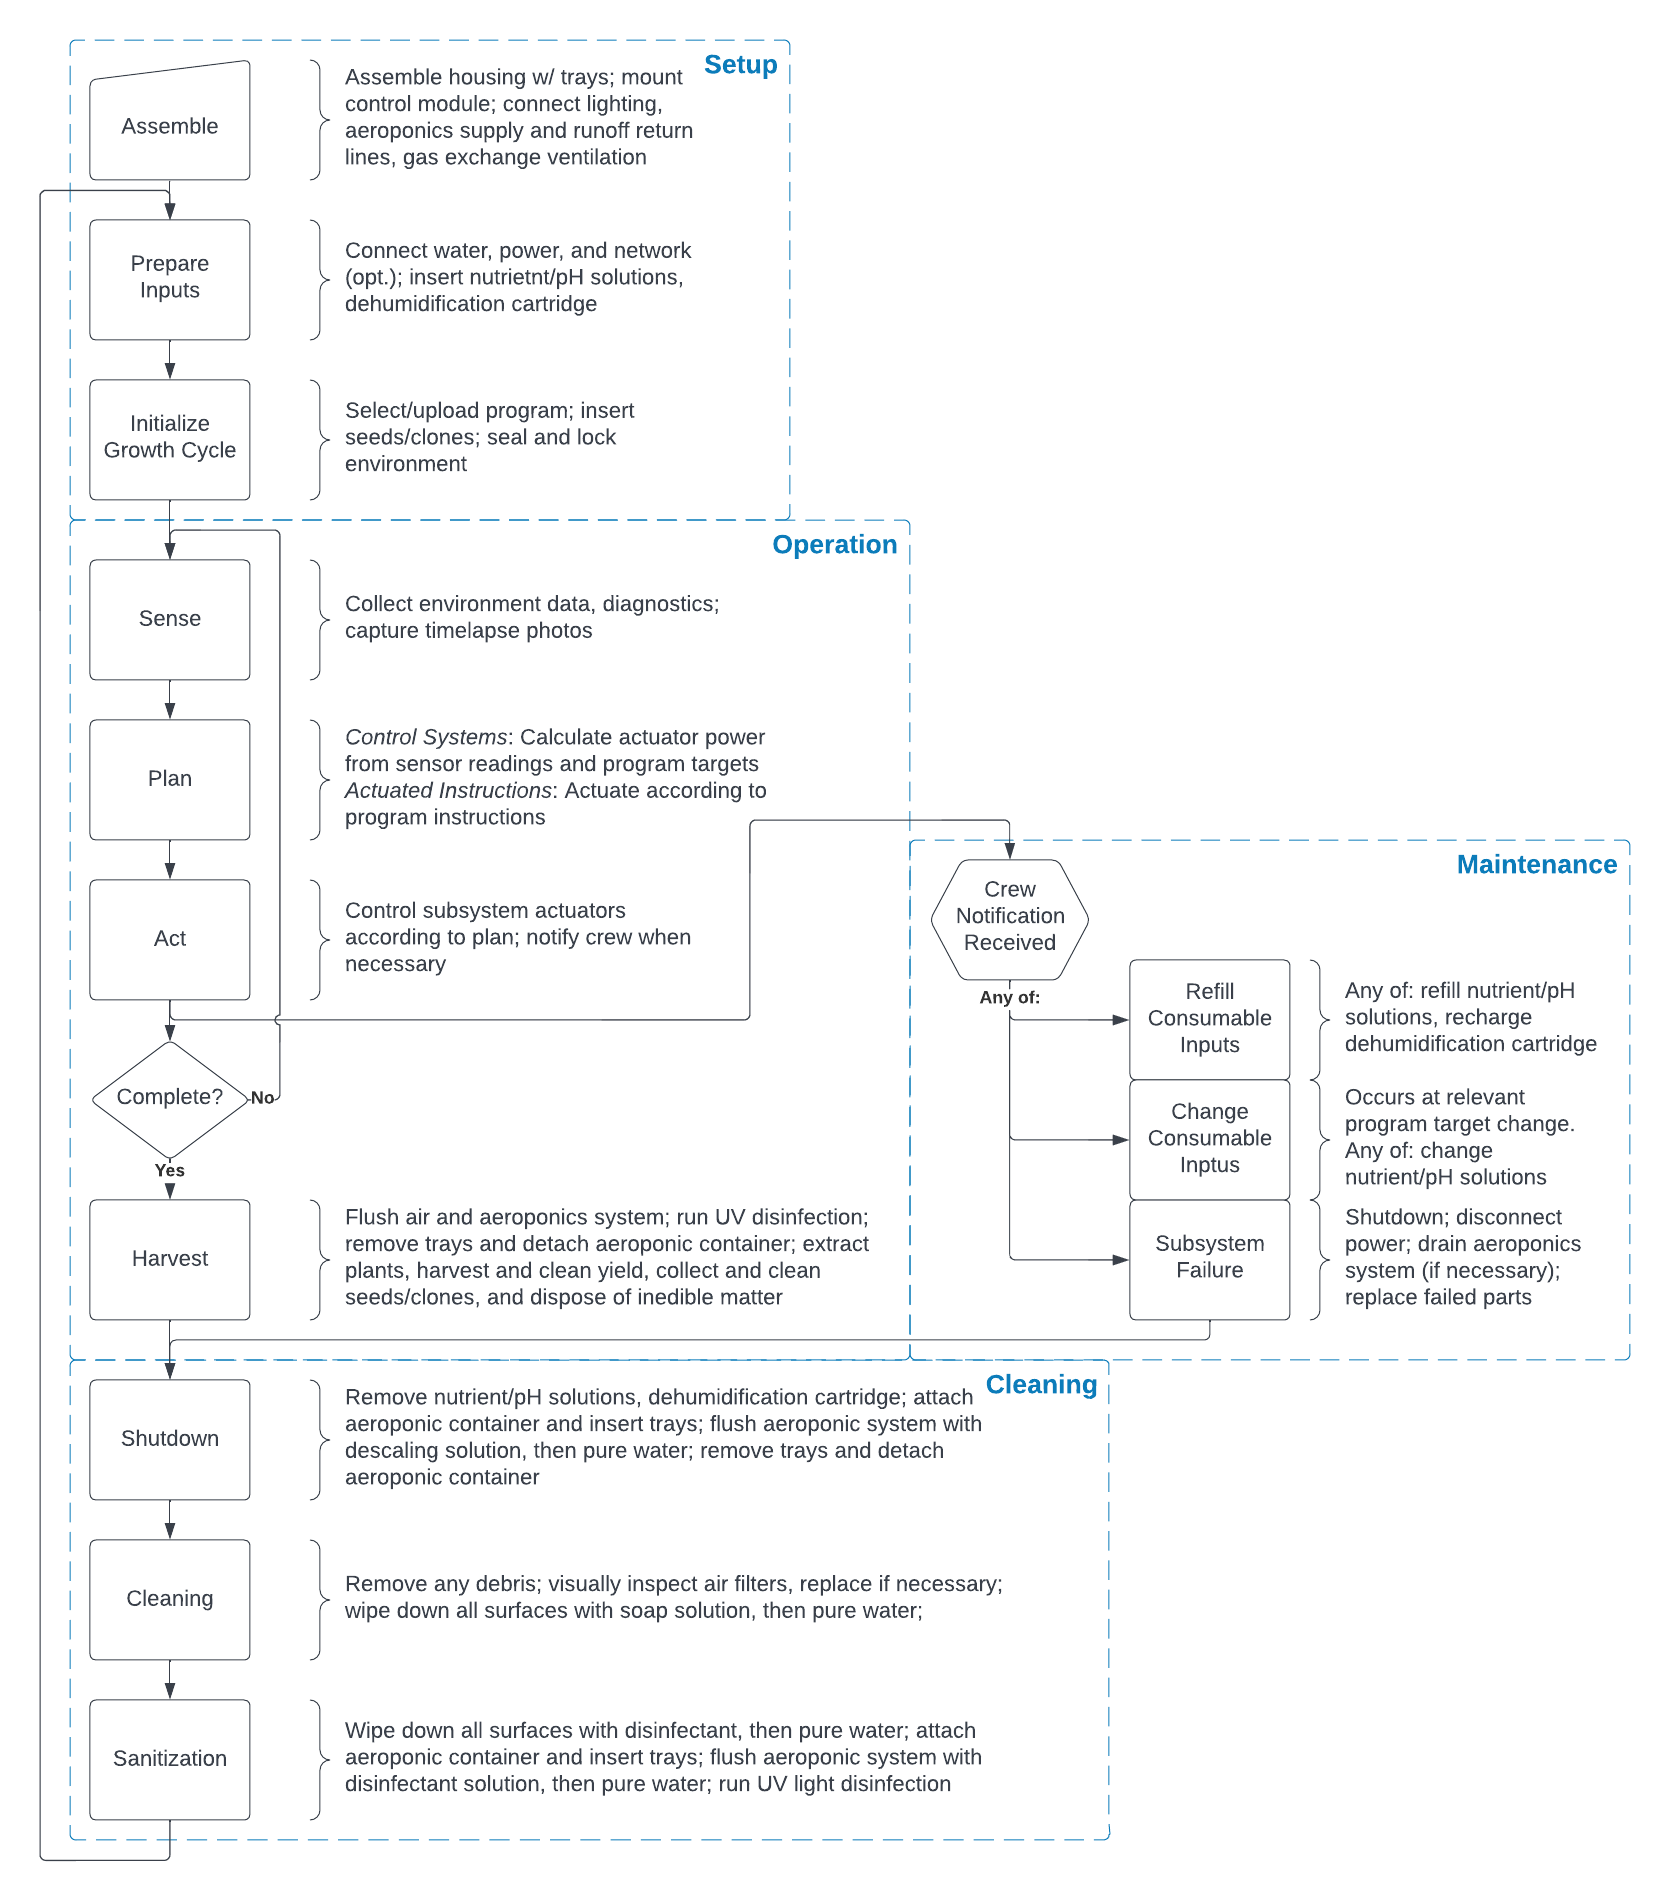
\includegraphics[width=0.9\textwidth]{../assets/figures/process.png}}
    \caption{Process diagram.}
    \label{fig:process}
\end{figure}

\clearpage

\subsubsection{Setup}
\label{sec:process_setup}

\textbf{Assembly}:
\begin{enumerate}
    \item Assemble housing, trays (see \ref{sec:housing});
    \item Mount control module, trays (see \ref{sec:housing});
    \item Connect subsystems to control module:
    \begin{itemize}
        \item \textit{Housing Solenoid Lock}: relay (see \ref{sec:housing})
        \item \textit{Aeroponics Supply \& Runoff Collection Lines}: quick-disconnect (see \ref{sec:aeroponics})
        \item \textit{Lighting Driver Board}: power, control signal (see \ref{sec:lighting})
    \end{itemize}
    \item Connect gas exchange exhaust to ventilation (see \ref{sec:gas});
\end{enumerate}

\textbf{Prepare Inputs}:
\begin{enumerate}
    \item Connect supply inputs:
    \begin{itemize}
        \item \textit{Power}: 120V 60Hz AC (see \ref{sec:automation});
        \item \textit{Network}: ethernet or wireless, optional (see \ref{sec:automation})
        \item \textit{Water}: reverse-osmosis, ambient (see \ref{sec:aeroponics})
    \end{itemize}
    \item Insert consumable inputs:
    \begin{itemize}
        \item \textit{Nutrient/pH Adjusment Solutions}: pouches (see \ref{sec:aeroponics})
        \item \textit{Dehumidification Cartridge}: recharged (see \ref{sec:dehumidification})
    \end{itemize}
\end{enumerate}

\textbf{Initialize Growth Cycle}:
\begin{enumerate}
    \item Select or upload program;
    \item Insert seeds/clones;
    \item Seal and lock environment;
    \item Start growth cycle;
\end{enumerate}

\textbf{Proceed to Operation} (see \ref{sec:process_operation}).

\subsubsection{Operation}
\label{sec:process_operation}

\textbf{Sense, Plan, Act} represent the three simultaneous automatic processes of the program's execution (see \ref{sec:automation}).

\textbf{Sense}:
Environment data, diagnostic information, and timelapse photos are captured and stored at regular intervals;

\textbf{Plan}:\\
\textit{Control Systems}: Actuator controls are calculated from sensor readings and program targets.\\
\textit{Actuated Instructions}: Actuator controls are derived from program instructions.

\textbf{Act}:
Subsystem actuators are controlled according to plan. Crew is notified to refill consumable inputs when low, change consumable inputs on program target change, and on any subsystem failure (see \ref{sec:process_maintenance}), as well as when to harvest and on End of Program (EoP).

\clearpage

\textbf{Harvest and/or EoP}:
\begin{enumerate}
    \item All air is exhausted (automatic, see \ref{sec:gas});
    \item Flush aeroponics system with pure water (automatic, see \ref{sec:aeroponics});
    \item Run UV disinfection (automatic, see \ref{sec:lighting});
    \item Unlock and open environment;
    \item Remove trays (see \ref{sec:housing}) and detach aeroponic container (see \ref{sec:aeroponics});
    \item \textbf{If EoP}: Extract plants;
    \item Harvest and clean yield;
    \item Collect, clean, and store seeds/clones;
    \item \textbf{If EoP}: Dispose of inedible matter;
\end{enumerate}

\textbf{If EoP, proceed to Cleaning} (see \ref{sec:process_cleaning})\textbf{. Otherwise, seal and lock environment and resume program.}

\subsubsection{Maintenance}
\label{sec:process_maintenance}

\textbf{Notification Handling}:
\begin{itemize}
    \item \textit{Refill Consumable Inputs}: includes refilling nutrient/pH adjustment solutions (see \ref{sec:aeroponics}), recharging the dehumidification cartridge (see \ref{sec:dehumidification})
    \item \textit{Change Consumable Inputs}: includes changing nutrient/pH adjustment solutions (see \ref{sec:aeroponics})
    \item \textit{Subsystem Failure}: all operation stopped, proceed to \textit{Shutdown} (see \ref{sec:process_cleaning}), disconnect power (see \ref{sec:automation}), then drain aeroponics system if necessary (see \ref{sec:aeroponics}) and replace failed components
\end{itemize}

\subsubsection{Cleaning}
\label{sec:process_cleaning}

\textbf{Shutdown}:
\begin{enumerate}
    \item Remove nutrient/pH solutions (see \ref{sec:aeroponics}), dehumidification cartridge (see \ref{sec:dehumidification});
    \item Attach aeroponic container (see \ref{sec:aeroponics}) and insert trays (see \ref{sec:housing});
    \item Flush aeroponic system with descaling solution (see \ref{sec:aeroponics});
    \item Flush aeroponic system with pure water (see \ref{sec:aeroponics});
    \item Remove trays (see \ref{sec:housing}) and detach aeroponic container (see \ref{sec:aeroponics});
\end{enumerate}

\textbf{Cleaning}:
\begin{enumerate}
    \item Visually inspect all surfaces for debris (remove) and components for damage (replace);
    \item Visually inspect all air filters (see \ref{sec:dehumidification}, \ref{sec:gas}), replace if necessary;
    \item Wipe down all surfaces with soap solution;
    \item Wipe down all surfaces with pure water;
\end{enumerate}

\textbf{Sanitization}:
\begin{enumerate}
    \item Wipe down all surfaces with disinfectant solution;
    \item Wipe down all surfaces with pure water;
    \item Dry all surfaces;
    \item Attach aeroponic container (see \ref{sec:aeroponics}) and insert trays (see \ref{sec:housing});
    \item Flush aeroponic system with disinfectant solution (see \ref{sec:aeroponics});
    \item Flush aeroponic system with pure water (see \ref{sec:aeroponics});
    \item Seal and lock environment;
    \item Run UV sanitization (\ref{sec:lighting});
\end{enumerate}

\textbf{Proceed to Prepare Inputs} (see \ref{sec:process_setup}).

% Stability: Demonstrate the stability of both the input products used and food product outputs and provide rationalization of the estimated time the inputs and outputs will be fit for use and/or consumption (i.e., shelf-life). (limit 8000 characters)

\newpage

% References
\bibliographystyle{IEEEtran}
\bibliography{references}
\end{document}